\chapter{Modules}
\label{sec:mods}
%%%%%%%%%%%%%%%%%%%%%%%%%%%%%%%%%%%%%%%%%%%%%%%%%%%%%%%%%
We list the individual modules of the ontology, together with their axioms and explanations thereof. Each axiom is listed only once (for now), i.e. some axioms pertaining to a module may be found in the axiom set listed for an earlier listed module. Schema diagrams are provided throughout, but the reader should keep in mind that while schema diagrams are very useful for understanding an ontology \cite{odp-documentation,ShimizuEKHKH19}, they are also inherently ambiguous.

%%%%%%%%%%%%%%%%%%%%%%%%%%%%%%%%%%%%%%%%%%%%%%%%%%%%%%%%
%\section{Module Overview}
%\label{ssec:modules}
%%%%%%%%%%%%%%%%%%%%%%%%%%%%
The following are the modules which together constitute our partial ontology for some track and trace use cases within the agricultural industry.\footnote{Supported and worked scenarios (e.g. filling of containers, field operations, grain storage and distribution, testing, drying, blending, and shipment within the food supply chain) can be found in our supplementary documents located here. See \url{document}.} Each of them will be presented in detail further below.
\begin{description}
    \item[TRU] 
    \item[Containers]
    \item[Identifier]
    \item[Trajectory]
    \item[Quantity of Material]
    \item[Master Event] with these specialized sub-modules
    \begin{description}
        \item[Transfer Event] 
        \item[Transformation Event] 
        \item[Custody Change Event] 
        \item[Owner Change Event] 
        \item[Transport Event] 
        \item[Observation Event] 
    \end{description}
\end{description}
Before we discuss each of them in turn, let us provide a partial overview of the modules. This is given in Figure \ref{fig:agri_overview}; a much more complete diagram can be found in Chapter \ref{chap:all}. Central to our  modeling are the notions of (1) Traceable Resource Unit (TRU, Section \ref{ssec:tru}), which is an amount of material with an identifier, that is moving along the supply chain, (2) Events (Section \ref{ssec:master}) which are relevant for  tracing TRUs, and (3) Containers (Section \ref{ssec:containers}) which hold the TRUs, e.g. for transport. Both TRUs and Containers participate in Events in various roles (appropriate to the specific type of Event). Containers and TRUs may move along trajectories. 

\begin{figure}[ptb]
\begin{center}
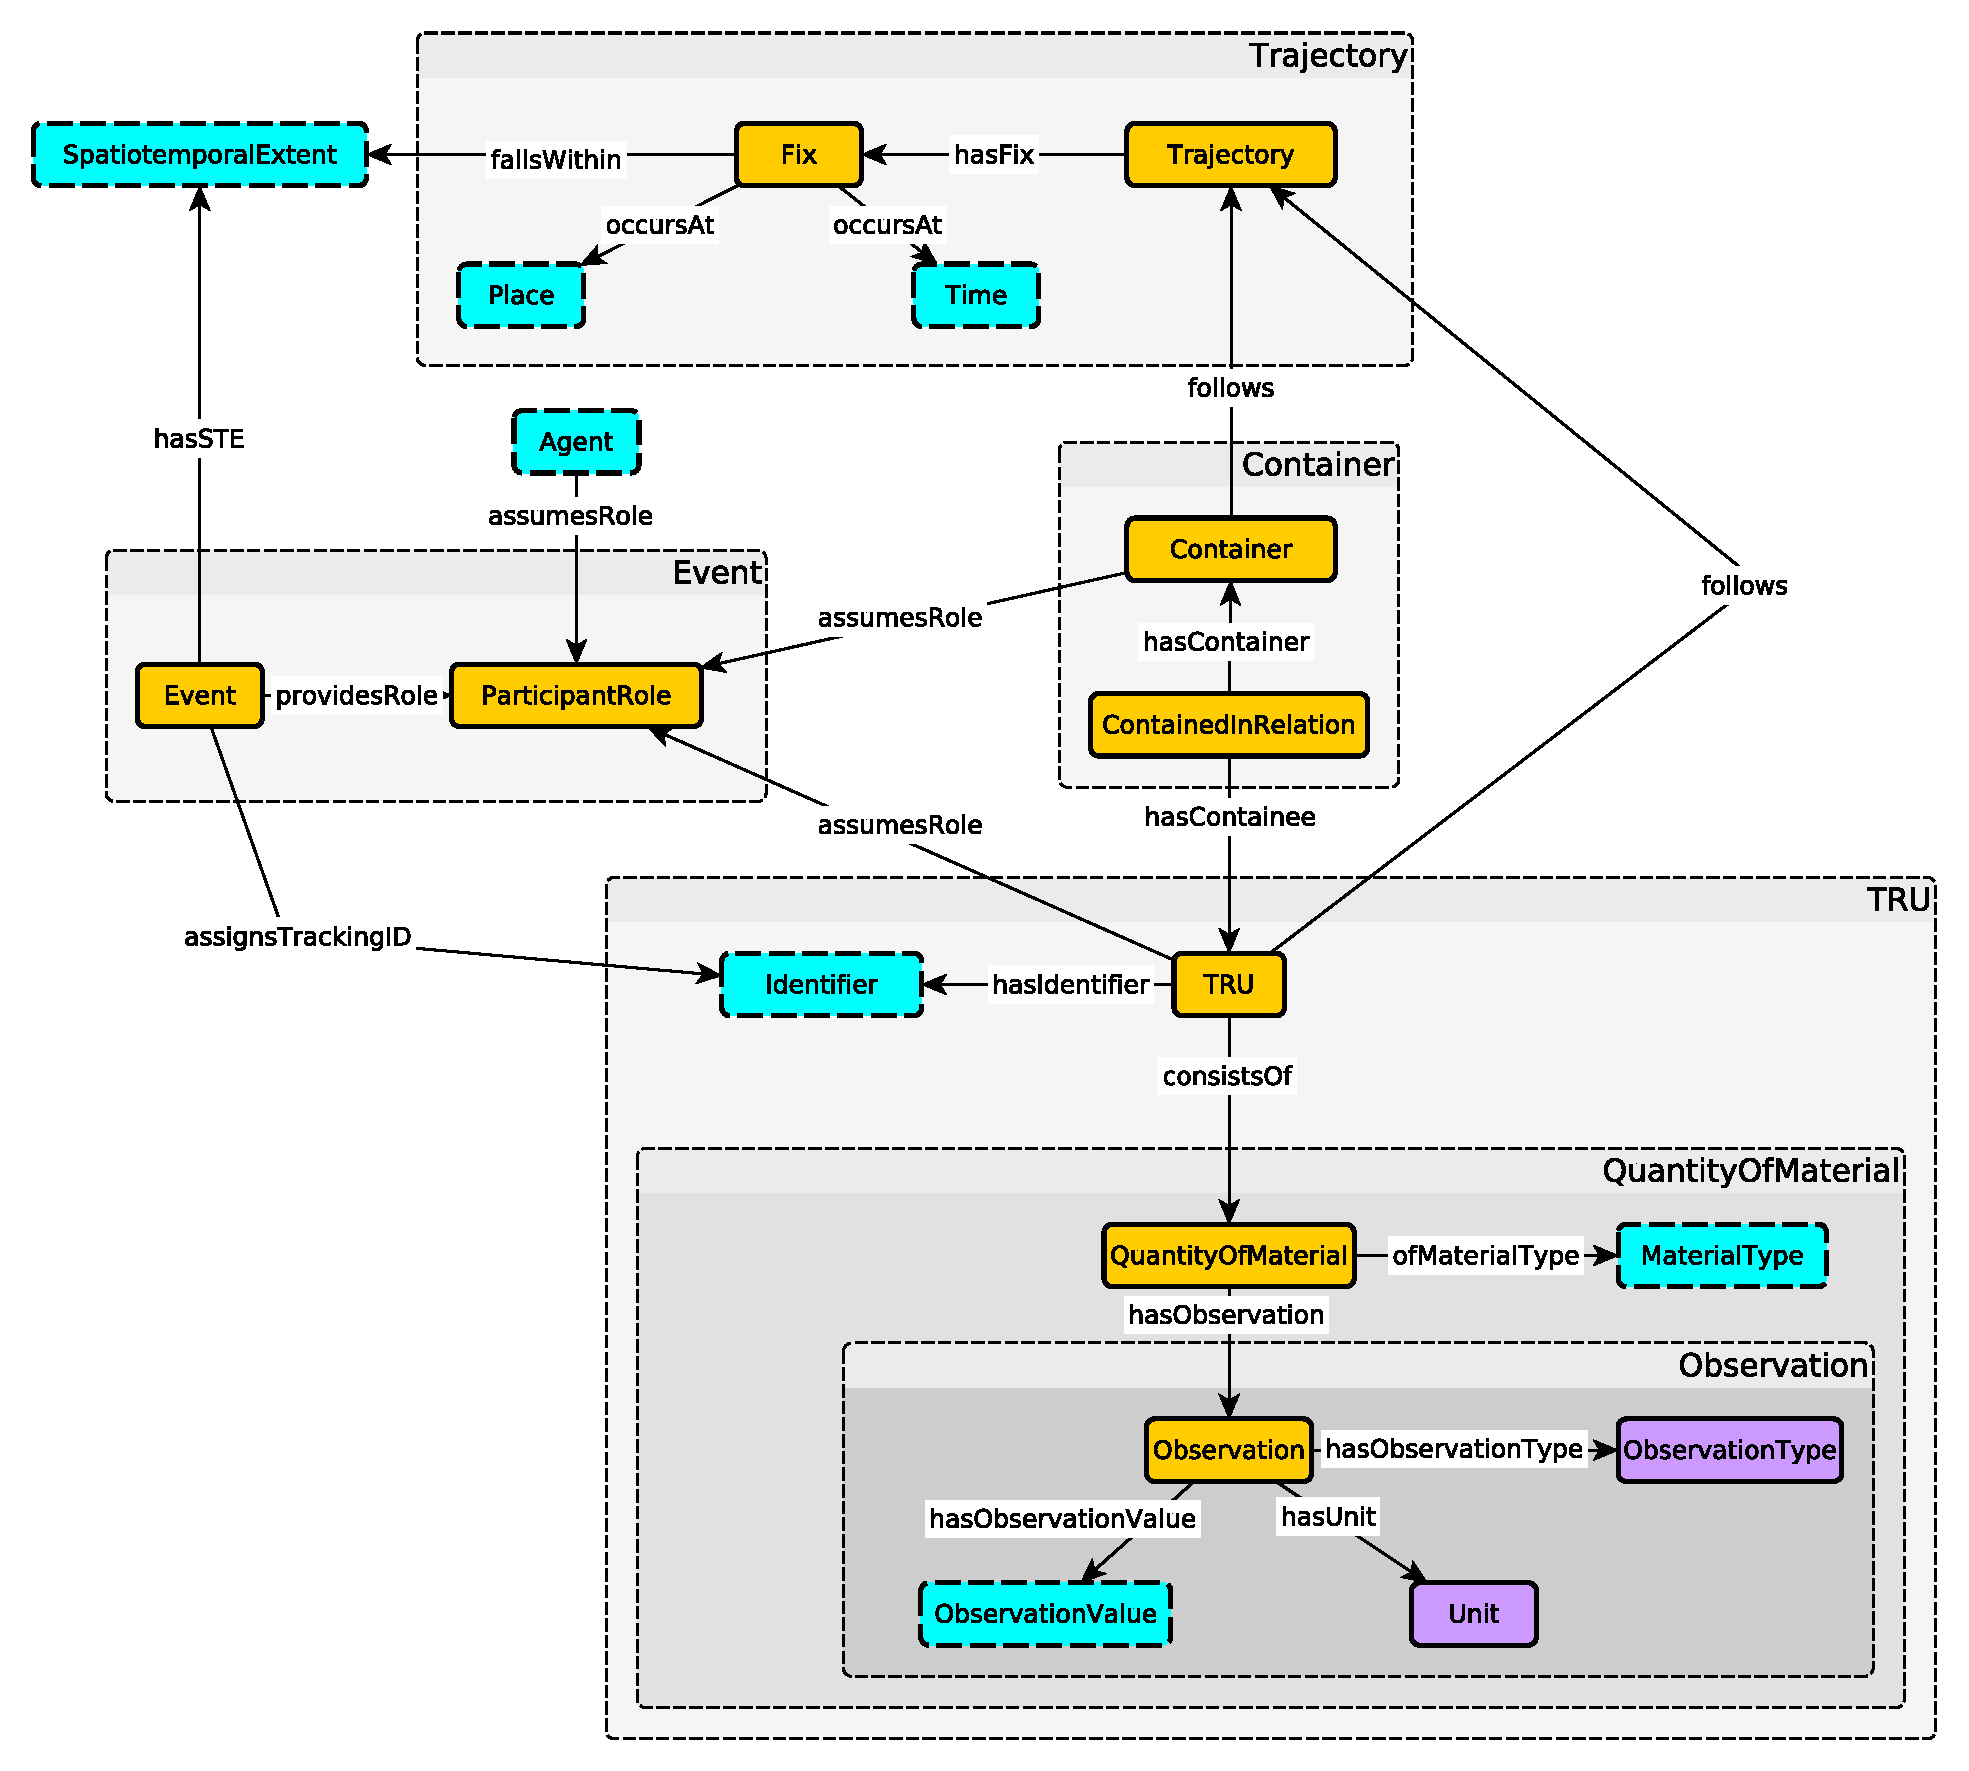
\includegraphics[width=\textwidth]{diagrams/agri_overview}
\end{center}
\caption{Overview of interconnected modules.}
\label{fig:agri_overview}
\end{figure}

\newpage

%%%%%%%%%%%%%%%%%%%%%%%%%%%%%%%%%%%%%%%%%%%%%%%%%%%%%%%%
\section{TRU}
\label{ssec:tru}
%%%%%%%%%%%%%%%%%%%%%%%%%%%%
\begin{figure}[h!]
\begin{center}
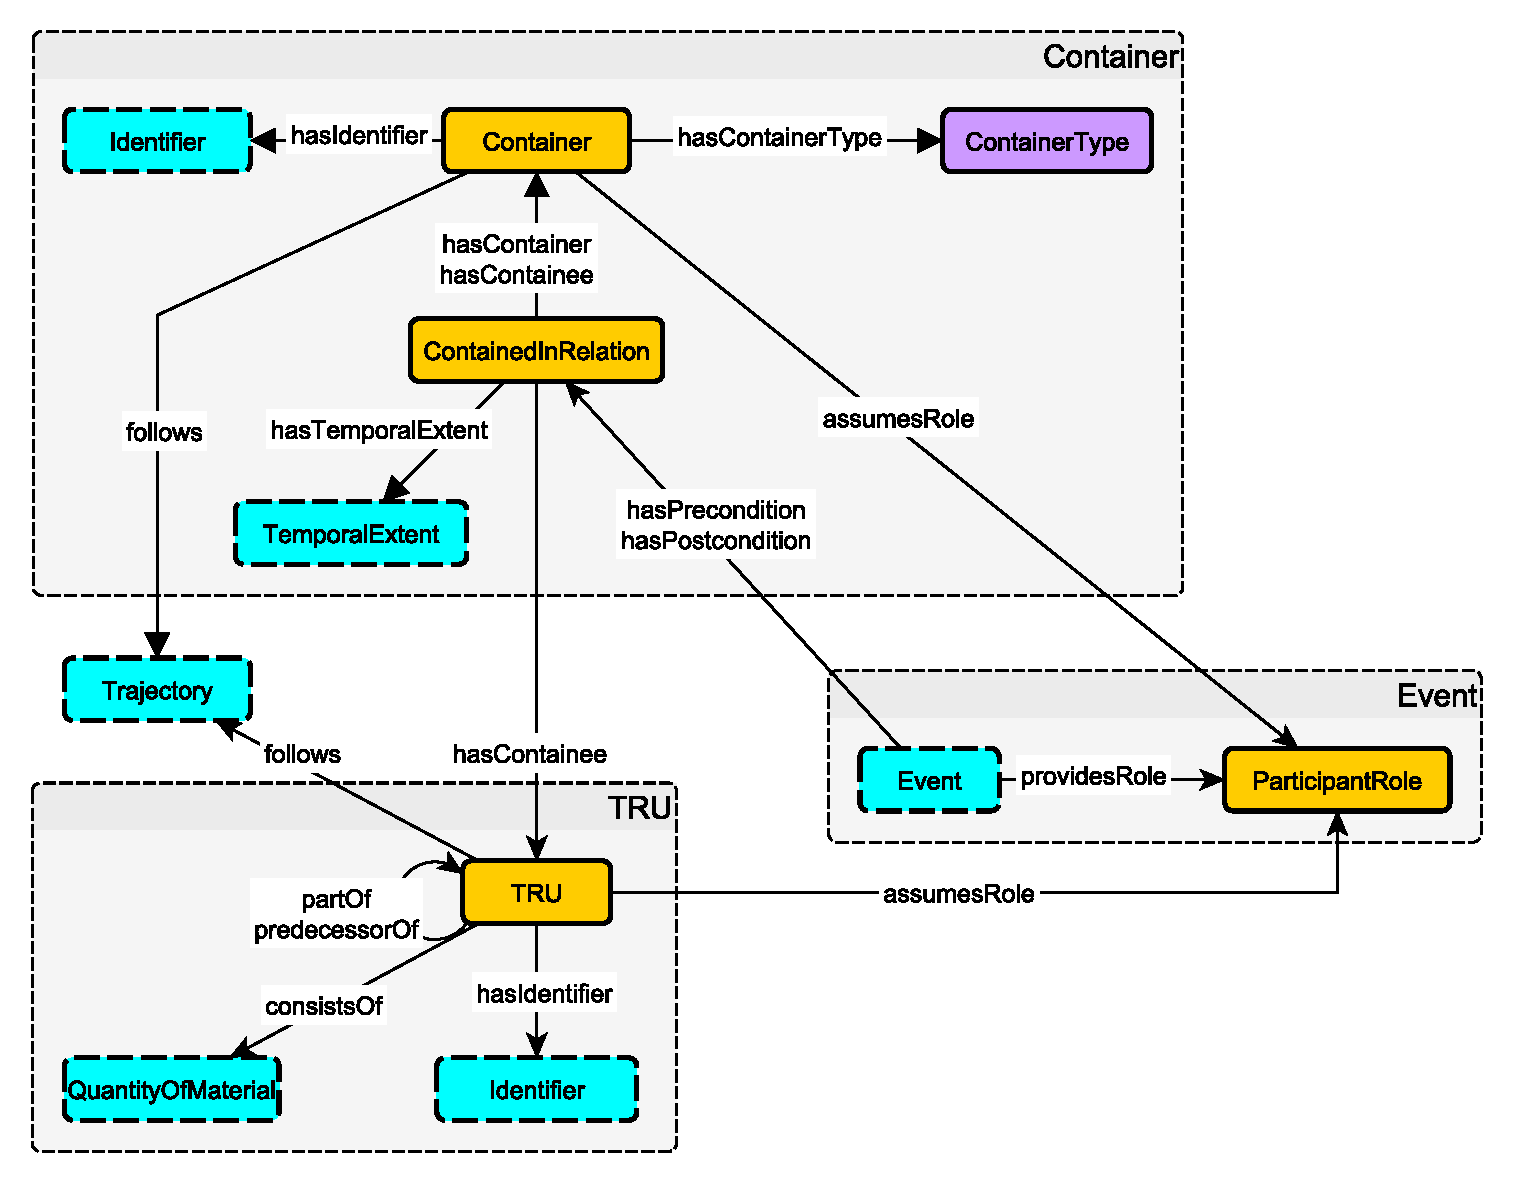
\includegraphics[width=.9\textwidth]{diagrams/tru}
\end{center}
\caption{Schema Diagram for the TRU and Container modules. Note that the Event module is only partially depicted.}
\label{fig:tru}
\end{figure}
%%%%%%%%%%%%%%%%%%%%%%%%%%%%
A Traceable Resource Unit (TRU) consists of a quantity of something (e.g. wheat grain) of interest, together with one of several identifiers for the TRU. TRUs are considered to be in containers (more about containers below in Section \ref{ssec:containers}) and participate in Events relevant to tracing, in appropriate roles. TRUs can be part of other TRUs, and we have a predecessorOf relation between TRUs, relevant to tracing.

A schema diagram is given in Figure \ref{fig:tru} on the lower left. The diagram also contains a diagram for the Container module (top) which we will discuss next. The Event module is only very partially depicted and will be spelled out in more detail further below.

\subsubsection*{Axioms:}
\begin{align}
    \textsf{TRU} &\sqsubseteq \mathord{\geq}0 \textsf{partOf.TRU}\\
    \textsf{TRU} &\sqsubseteq \mathord{\geq}0 \textsf{predecessorOf.TRU}\\
    \textsf{TRU} &\sqsubseteq \forall\textsf{hasIdentifier.Identifier}\\
    \textsf{TRU} &\sqsubseteq \exists\textsf{hasIdentifier.Identifier}\\
    \textsf{Identifier} &\sqsubseteq \mathord{\leq} 1\textsf{hasIdentifier}\mathord{^-}.\top\\
    \textsf{TRU} &\sqsubseteq \forall\textsf{consistsOf.QuantityOfMaterial}\\
    \textsf{TRU} &\sqsubseteq \mathord{\leq} 1 \textsf{consistsOf}.\top\\
    \textsf{TRU} &\sqsubseteq \exists\textsf{consistsOf.QuantityOfMaterial}\\
    \textsf{TRU} &\sqsubseteq \forall\textsf{assumesRole.ParticipantRole}\\
    \textsf{TRU} &\sqsubseteq \forall\textsf{follows.Trajectory}\\
    \textsf{TRU} &\sqsubseteq \exists\textsf{follows.Trajectory}\\
    \textsf{TRU} &\sqsubseteq \exists\textsf{hasContainee}^-.\textsf{ContainedInRelation}\\
    \textsf{prececessorOf} \circ \textsf{predecessorOf} &\sqsubseteq \textsf{predecessorOf}
\end{align}

\subsubsection*{Axiom Explanations:}
\begin{enumerate}
    \item Structural Tautology: A \textsf{TRU} may be \textsf{partOf} another \textsf{TRU}.
    \item Structural Tautology: A \textsf{TRU} may be a \textsf{predecessorOf} of another \textsf{TRU}.
    \item Scoped Range: The range of \textsf{hasIdentifier} is \textsf{Identifier}, scoped by \textsf{TRU}.
    \item Existential: A \textsf{TRU} has a least one \textsf{Identifier}.
    \item Inverse Scoped Functionality: An \textsf{Identifier} identifies at most one thing.
    \item Scoped Range: The range of \textsf{consistsOf} is \textsf{QuantityOfMaterial}, scoped by \textsf{TRU}.
    \item Scoped Functionality: \textsf{consistsOf} is functional, scoped by \textsf{TRU}.
    \item Existential: A \textsf{TRU} consists of at least one \textsf{QuantityOfMaterial}.
    \item Scoped Range: The range of \textsf{assumesRole} is \textsf{ParticipantRole}, scoped by \textsf{TRU}.
    \item Scoped Range: The range of \textsf{follows} is \textsf{Trajectory}, scoped by \textsf{TRU}.
    \item Existential: A \textsf{TRU} follows a \textsf{Trajectory}.
    \item Inverse Existential: A \textsf{ContainedInRelation} refers to at most one \textsf{TRU}.
    \item Transitivity: \textsf{predecessorOf} is transitive.
\end{enumerate}

\subsubsection*{Remarks:}
\begin{enumerate}
    \item A \textsf{TRU} always has an identifier (even though it may not be known); a \textsf{TRU} may have several identifiers. 
    \item A \textsf{TRU} is always contained in at least one container (even though it may not be known or an unusual type of container, such as a (part of a) field. Since containers can be in other containers, a \textsf{TRU} can be in several containers.
    \item The \textsf{ContainedInRelation} is discussed and axiomatized further in Section \ref{ssec:containers}.
\end{enumerate}

\subsubsection*{Questions:}
\begin{enumerate}
    \item Should the \textsf{partOf} relationship be replaced with a more  appropriate appropriate version from \cite{MODL}, in which case it could then be declared transitive? The question is: which of those types? Probably member-collection. But could also be portion-mass or stuff-object?
\end{enumerate}

%%%%%%%%%%%%%%%%%%%%%%%%%%%%%%%%%%%%%%%%%%%%%%%%%%%%%%%%
\section{Container}
\label{ssec:containers}
%%%%%%%%%%%%%%%%%%%%%%%%%%%%
In our context, by Container we mean anything that can hold TRUs, i.e., we use the term in a rather abstract sense. A container may even be stationary (such as a grain elevator), moving in a continuous manner (such as a harvester/combine) or even lack a physical enclosure (such as a grain field which is then defined by its geospatial polygon boundary). At the same time, for our use case, we do not need to be very specific about Containers: they carry identifiers, contain TRUs, and follow trajectories. 

\begin{figure}[tb]
\begin{center}
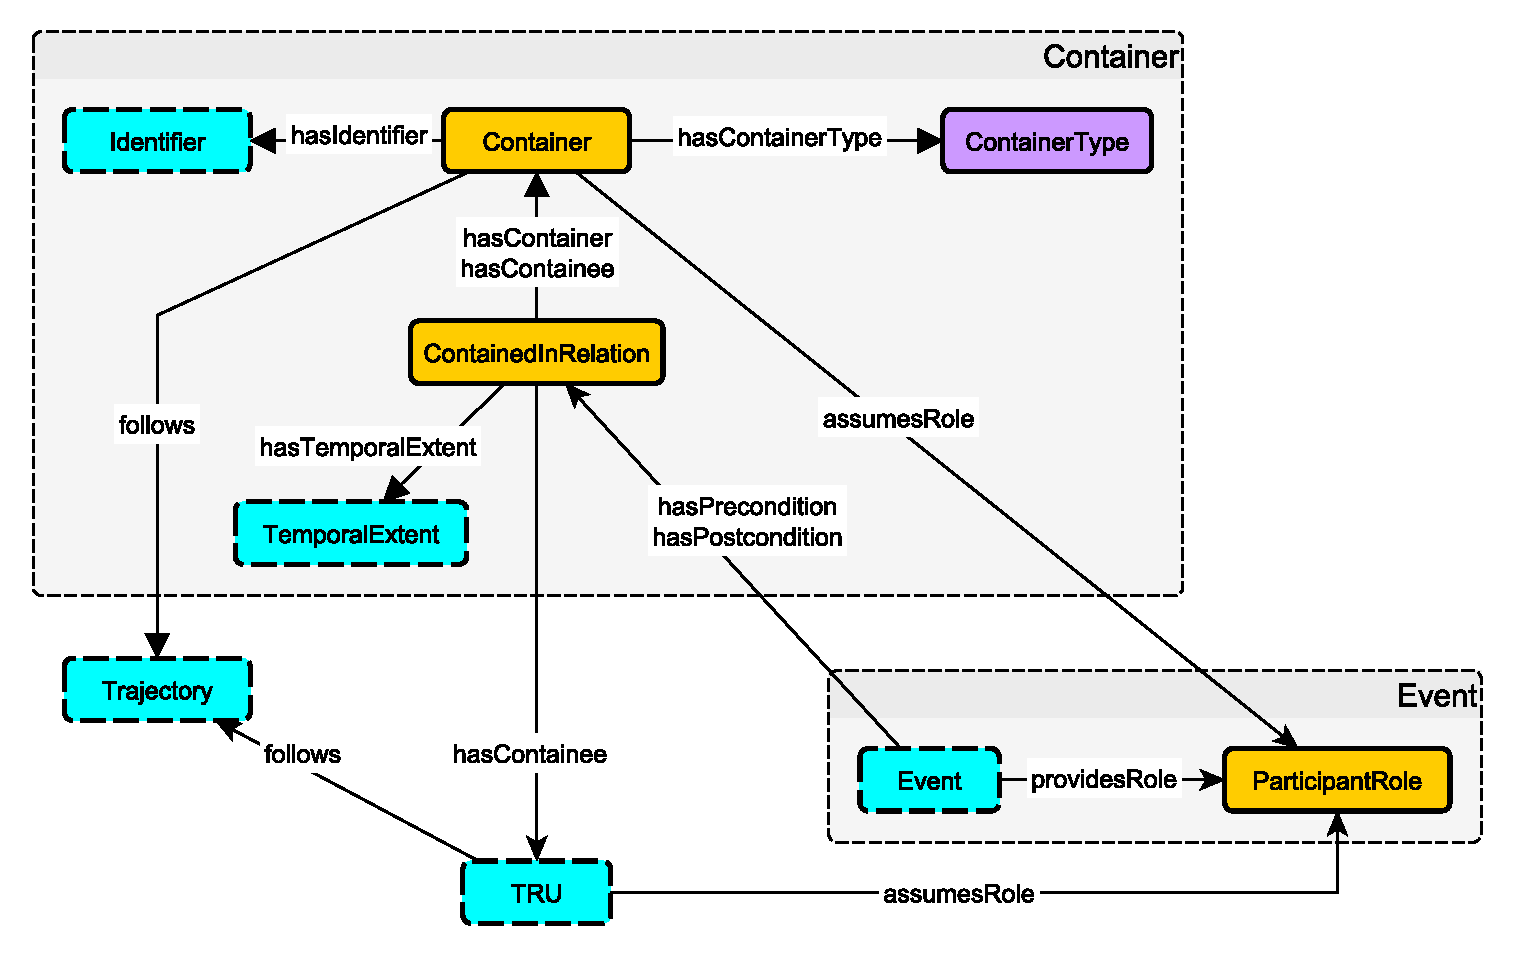
\includegraphics[width=\textwidth]{diagrams/container}
\end{center}
\caption{Schema Diagram for the Container module}
\label{fig:Containers}
\end{figure}

\subsubsection*{Axioms:}

\begin{align}
    \textsf{Container} &\sqsubseteq \forall\textsf{follows.Trajectory}\\
    \textsf{Container} &\sqsubseteq \exists\textsf{follows.Trajectory}\\
    \textsf{Container} &\sqsubseteq \forall\textsf{hasIdentifier.Identifier}\\
    \textsf{Container} &\sqsubseteq \exists\textsf{hasIdentifier.Identifier}\\
    \textsf{Identifier} &\sqsubseteq \mathord{\leq} 1\textsf{hasIdentifier}\mathord{^-}.\top\\
    \top &\sqsubseteq \forall\textsf{hasContainerType.ContainerType}\\
    \exists\textsf{hasContainerType}.\top &\sqsubseteq \textsf{Container}\\
    \textsf{Container} &\sqsubseteq \exists\textsf{hasContainerType.ContainerType}\\
    \textsf{Container} &\sqsubseteq \mathord{\geq}0\textsf{assumesRole.ParticipantRole}\\
    \exists\textsf{hasContainer}.\top &\sqsubseteq \textsf{ContainedInRelation}\\
    \top &\sqsubseteq \forall\textsf{hasContainer.Container}\\
    \exists\textsf{hasContainee}.\top &\sqsubseteq \textsf{ContainedInRelation}\\
    \textsf{ContainedInRelation} &\sqsubseteq \exists\textsf{hasContainee}.\top\\
    \textsf{ContainedInRelation} &\sqsubseteq \exists\textsf{hasContainer}.\top\\
    \textsf{ContainedInRelation} &\sqsubseteq \mathord{\geq}0\textsf{hasContainee}.(\textsf{Container} \sqcup \textsf{TRU})\\
    \top &\sqsubseteq \forall\textsf{hasTemporalExtent.TemporalExtent}\\
    \textsf{ContainedInRelation} &\sqsubseteq \exists\textsf{hasTemporalExtent.TemporalExtent}
\end{align}

\subsubsection*{Axiom Explanations:}

\begin{enumerate}
    \item Scoped Range: The range of \textsf{follows} is \textsf{Trajectory}, scoped by \textsf{Container}.
    \item Existential: A \textsf{Container} \textsf{follows} a \textsf{Trajectory}.
    \item Scoped Range: The range of \textsf{hasIdentifier} is \textsf{Identifier}, scoped by \textsf{Container}.
    \item Existential: A \textsf{Container} has an \textsf{Identifier}.
    \item Inverse Scoped Functionality: An \textsf{Identifier} identifies at most one thing.
    \item Range: The range of \textsf{hasContainerType} is \textsf{ContainerType}.
    \item Domain: The domain of \textsf{hasContainerType} is \textsf{Container}.
    \item Existential: hasContainerType
    \item Structural Tautology: A \textsf{Container} may assume a \textsf{ParticipantRole}.
    \item Domain: The domain of \textsf{hasContainer} is \textsf{ContainedInRelation}.
    \item Range: The range of \textsf{hasContainer} is \textsf{Container}.
    \item Domain: The domain of \textsf{hasContainee} is \textsf{ContainedInRelation}.
    \item Existential: A \textsf{ContainedInRelation} has some containee.
    \item Existential: A \textsf{ContainedInRelation} has some container. 
    \item Structural Tautology: A \textsf{ContainedInRelation} may have a containee that is a \textsf{Container} or \textsf{TRU}.
    \item Range: The range of \textsf{hasTemporalExtent} is \textsf{TemporalExtent}.
    \item Scoped Existential: A \textsf{ContainedInRelation} has a \textsf{TemporalExtent}.
\end{enumerate}

\subsubsection*{Remarks:}
\begin{itemize}
    \item We would like to state that a container cannot be in two places at the same time, but it is not clear at this stage whether that can be done in OWL. To be revisited when looking at spatiotemporal extents.
    \item Every Container has a unique identifier, even though that identifier may be a very local reference (such as \emph{on the back parking lot}). The Identifier module details can reflect this.
    \item Trajectories of TRU and Container have to be compatible, as has the temporality of the ContainedInRelation.
    \item hasPre- and hasPostcondition axioms are included in the Event module description below.
    \item The contained-in relation has been reified in order to make it possible to record a temporal extent for it, and also (if relevant) that certain containment relations are relevant to certain types of critical tracking events, e.g. for the TransferEvent which is described further below. Furthermore, contained-in relations may be complex, e.g. it may be relevant whether contamination of a container can cause contamination of container content. By reifying the contained-in relation, it will be easier to extend the model when and if desired.
    \item It is possible to specify transitivity of the contained-in relation, using complex axioms, if desired.
\end{itemize}

%%%%%%%%%%%%%%%%%%%%%%%%%%%%%%%%%%%%%%%%%%%%%%%%%%%%%%%%
\section{Identifier}
\label{ssec:identifier}
%%%%%%%%%%%%%%%%%%%%%%%%%%%%
Identifiers are the labels or serial-number through which a TRU (Traceable Resource Unit) or Container can be traced in the supply chain. Identifiers have a type and representation; we also specify a sub-module \textsf{IdentifierEncoding} to represent encoding information for identifiers. 

Recall that purple boxes (as in Figure \ref{fig:Containers}) indicate that the class should be treated as a controlled vocabulary, and is particular to the use-case at hand. For example, entities in the class \textsf{IdentifierEncodingScheme} will be URIs that uniquely identify particular encoding schemes (such as, the DOI scheme for online documents). There is no need in our use case to provide further scheme information as part of the ontology as, in general, these controlled vocabularies are structured and maintained by other organizations, and we can thus use these entities to point to their documentation.

% From Scott: Related to identifier types, many data exchange standards over the last 40 years have used this generic technique for identification to qualify an identifier with its type, including TDCC, ANSI ASC X12 Electronic Data Interchange, Open Applications Group OAGIS standard, GS1 barcoding standards, and more recently for field operations, the AgGateway ADAPT framework.  Each of these standards have a controlled vocabulary for identifier types, or provision to support a controlled vocabulary, but need to be further constrained by the business process context and resources available.  In the X12 case, used by FoodLogiQ for traceability, this code list has become massive over the years, and physically unmanageable except through industry or business to business agreement to manage a subset of these codes and contextual definitions. This alone has been one of the most challenging aspects of inter-operability and integration projects. Newer techniques to provide contextual definitions to code values based on the business process dimension has emerged.

\begin{figure}[tb]
\begin{center}
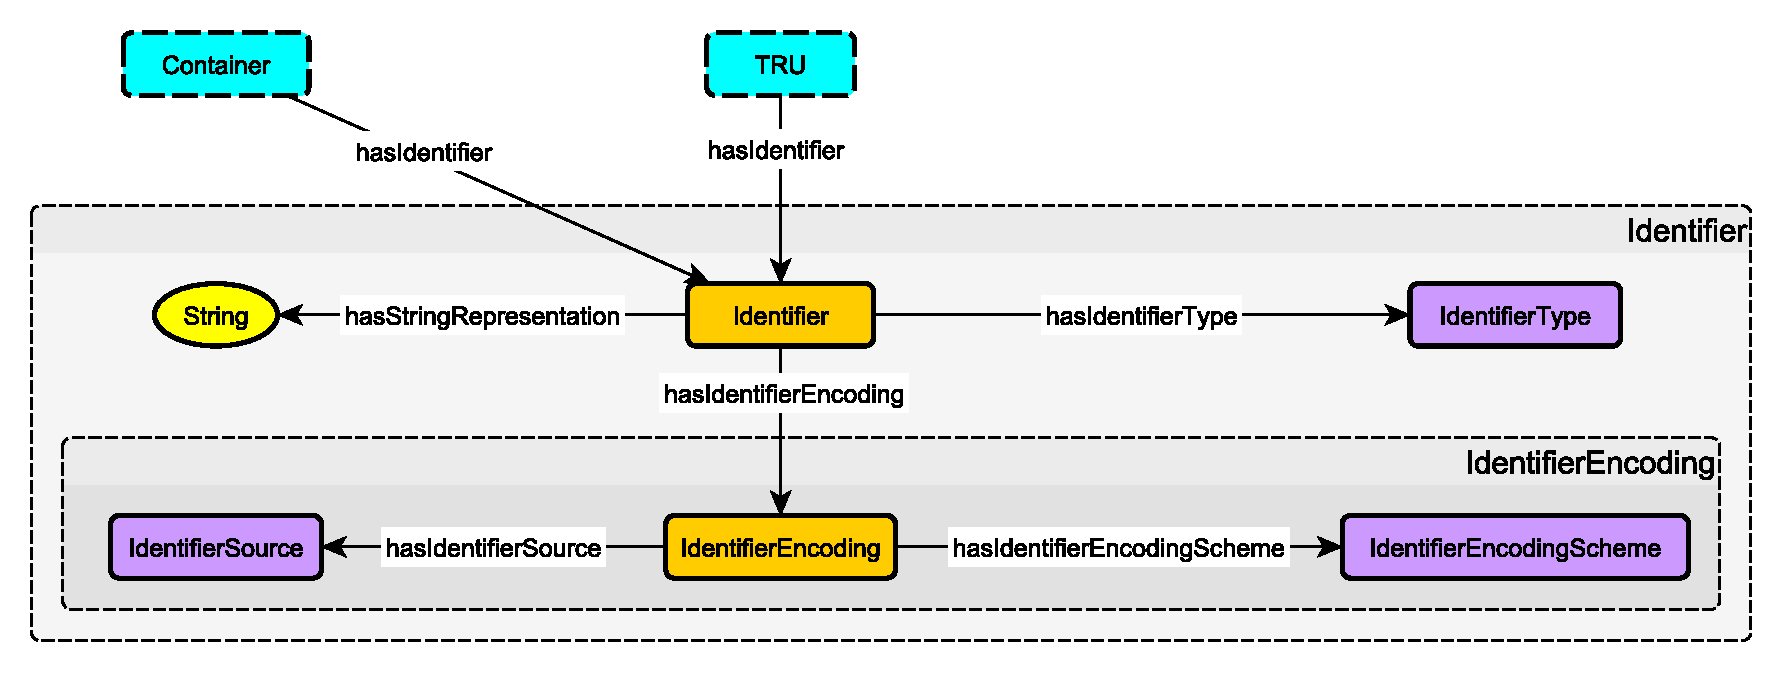
\includegraphics[width=\textwidth]{diagrams/identifier}
\end{center}
\caption{Schema Diagram for the Identifier module}
\label{fig:Identifier}
\end{figure}

\subsubsection*{Axioms:}
We use \textsf{hIES} in place of \textsf{hasIdentifierEncodingScheme}.
\begin{align}
    \textsf{TRU} &\sqsubseteq \forall\textsf{hasIdentifier.Identifier}\\
    \textsf{Identifier} &\sqsubseteq \mathord{\leq} 1\textsf{hasIdentifier}\mathord{^-}.\top\\
    \textsf{Identifier} &\sqsubseteq \forall\textsf{hasStringRepresentation.xsd:string}\\
    \textsf{Identifier} &\sqsubseteq \exists\textsf{hasStringRepresentation.xsd:string}\\
    \exists\textsf{hasIdentifierType.IdentifierType} &\sqsubseteq \textsf{Identifier}\\
    \textsf{Identifier} &\sqsubseteq \forall\textsf{hasIdentifierType.IdentifierType}\\
    \exists\textsf{hasIdentifierEncoding.IdentifierEncoding} &\sqsubseteq \textsf{Identifier}\\
    \textsf{Identifier} &\sqsubseteq \forall\textsf{hasIdentifierEncoding.IdentifierEncoding}\\
    \textsf{Identifier} &\sqsubseteq \exists\textsf{hasIdentifierEncoding.IdentifierEncoding}\\ 
    \exists\textsf{hasIdentifierSource.IdentifierSource} &\sqsubseteq \textsf{IdentifierEncoding}\\
    \textsf{IdentifierEncoding} &\sqsubseteq\forall \textsf{hasIdentifierSource.IdentifierSource}\\ 
    \textsf{IdentifierEncoding} &\sqsubseteq\exists\textsf{hasIdentifierSource.IdentifierSource}\\
    \exists\textsf{hIES.IdentifierEncodingScheme} &\sqsubseteq \textsf{IdentifierEncoding}\\
    \textsf{IdentifierEncoding}&\sqsubseteq\forall\textsf{hIES.IdentifierEncodingScheme} 
\end{align}

\subsubsection*{Axiom Explanations:}
\begin{enumerate}
    \item Scoped Range: The range of \textsf{hasIdentifier} is \textsf{Identifier}, scoped by \textsf{TRU}.
    \item Inverse Scoped Functionality: \textsf{hasIdentifier}
    \item Scoped Range: The range of \textsf{hasStringRepresentation} is \textsf{xsd:String}, scoped by \textsf{Identifier}.
    \item Existential: \textsf{hasStringRepresentation}
    \item Scoped Domain: The domain of \textsf{hasIdentifierType} is \textsf{Identifier}, scoped by \textsf{IdentifierType}.
    \item Scoped Range: The range of \textsf{hasIdentifierType} is \textsf{IdentifierType}, scoped by \textsf{Identifier}.
    \item Scoped Domain: The domain of \textsf{hasIdentifierEncoding} is \textsf{Identifier}, scoped by \textsf{IdentifierEncoding}.
    \item Scoped Range: The range of \textsf{hasIdentifierEncoding} is \textsf{IdentifierEncoding}, scoped by \textsf{Identifier}.
    \item Existential: \textsf{hasIdentifierEncoding}
    \item Scoped Domain: The domain of \textsf{hasIdentifierSource} is \textsf{IdentifierEncoding}, scoped by \textsf{IdentifierSource}.
    \item Scoped Range: The range of \textsf{hasIdentifierSource} is \textsf{IdentifierSource}, scoped by \textsf{IdentifierEncoding}.
    \item Existential: \textsf{hasIdentifierSource}
    \item Scoped Domain: The domain of \textsf{hasIdentifierEncodingScheme} is \textsf{IdentifierEncoding}, scoped by \textsf{IdentifierEncodingScheme}.
    \item Scoped Range: The range of \textsf{hasIdentifierEncodingScheme} is \textsf{IdentifierEncodingScheme}, scoped by \textsf{IdentifierEncoding}.
\end{enumerate}

%%%%%%%%%%%%%%%%%%%%%%%%%%%%%%%%%%%%%%%%%%%%%%%%%%%%%%%%
\section{Trajectory}
\label{ssec:trajectory}
%%%%%%%%%%%%%%%%%%%%%%%%%%%%
Trajectory is associated with the Container that is carrying something to be transported. In our modeling, a trajectory is essentially a sequence of Fixes in time and space. As such, a Fix occurs at some time and at some place. We also specify that a Fix falls within some spatiotemporal extent, which will be used to connect fixes with events.

This module is adapted from \cite{MODL}.

\begin{figure}[tb]
\begin{center}
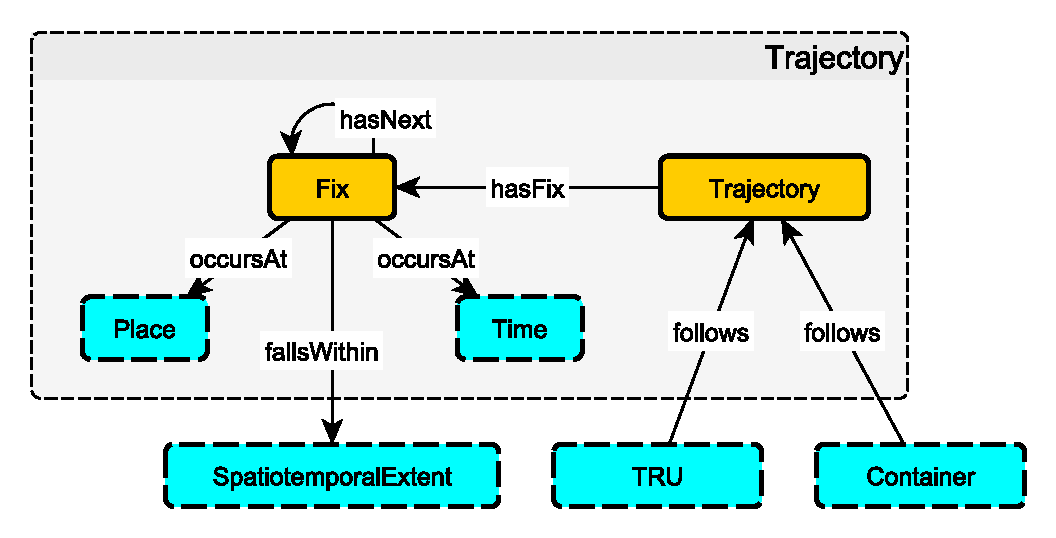
\includegraphics[width=.7\textwidth]{diagrams/trajectory}
\end{center}
\caption{Schema Diagram for the Trajectory module}
\label{fig:trajectory}
\end{figure}

\subsubsection*{Axioms:}
\begin{align}
    \textsf{Fix} &\sqsubseteq \exists\textsf{occursAt.Place}\\
    \textsf{Fix} &\sqsubseteq \exists\textsf{occursAt.Time}\\
    \exists\textsf{hasFix.Fix} &\sqsubseteq \textsf{Trajectory}\\
    \textsf{Trajectory} &\sqsubseteq \forall\textsf{hasFix.Fix}\\
    \textsf{Fix} &\sqsubseteq \mathord{\geq} 0\textsf{hasNext.Fix}\\
    \textsf{Fix} &\sqsubseteq \exists\textsf{fallsWithin.SpatiotemporalExtent}
\end{align}


\subsubsection*{Axiom Explanations:}
\begin{enumerate}
    \item Existential: A \textsf{Fix} must occur at a \textsf{Place}.
    \item Existential: A \textsf{Fix} must occur at a \textsf{Time}.
    \item Scoped Domain: The domain of \textsf{hasFix} is \textsf{Trajectory}, scoped by \textsf{Fix}.
    \item Scoped Range: The range of \textsf{hasFix} is \textsf{Fix}, scoped by \textsf{Trajectory}.
    \item Structural Tautology: A \textsf{Fix} may have a next \textsf{Fix}.
    \item Existential: A \textsf{Fix} must fall within a \textsf{SpatiotemporalExtent}.
\end{enumerate}

\subsubsection*{Remarks:}
\begin{itemize}
    \item There should be specified compatibility axioms between Place, Time, and SpatiotemporalExtent for Fixes, but this is likely outside the modeling capacities for OWL.
    \item Time (Trajectory module), TemporalScope (Container module) and SpatioTemporalExtent will have to be properly related when modeled.
\end{itemize}

%%%%%%%%%%%%%%%%%%%%%%%%%%%%%%%%%%%%%%%%%%%%%%%%%%%%%%%%
\section{Quantity of Material}
\label{ssec:quantity}
%%%%%%%%%%%%%%%%%%%%%%%%%%%%
In our context, a Quantity of Material refers to whatever constitutes the relevant commodity making up a TRU; e.g., a certain amount of grain. In this example grain would be the MaterialType (a separate submodule), and corresponding measurements (e.g., mass, volume, or humidity) providing information about it would be produced at ObservationEvents (see module below). 

Measurements (a submodule) come with a measurement type (such as, humidity, mass, length), and have a measurement value (which may be numeric, but could also be qualitative) and a unit (such as, meters or grams, or "numeric" for a count).

This module is adapted from \cite{MODL} -- in particular the Quantity pattern from \cite{MODL} has been generalized to the Measurement submodule.

\begin{figure}[tb]
\begin{center}
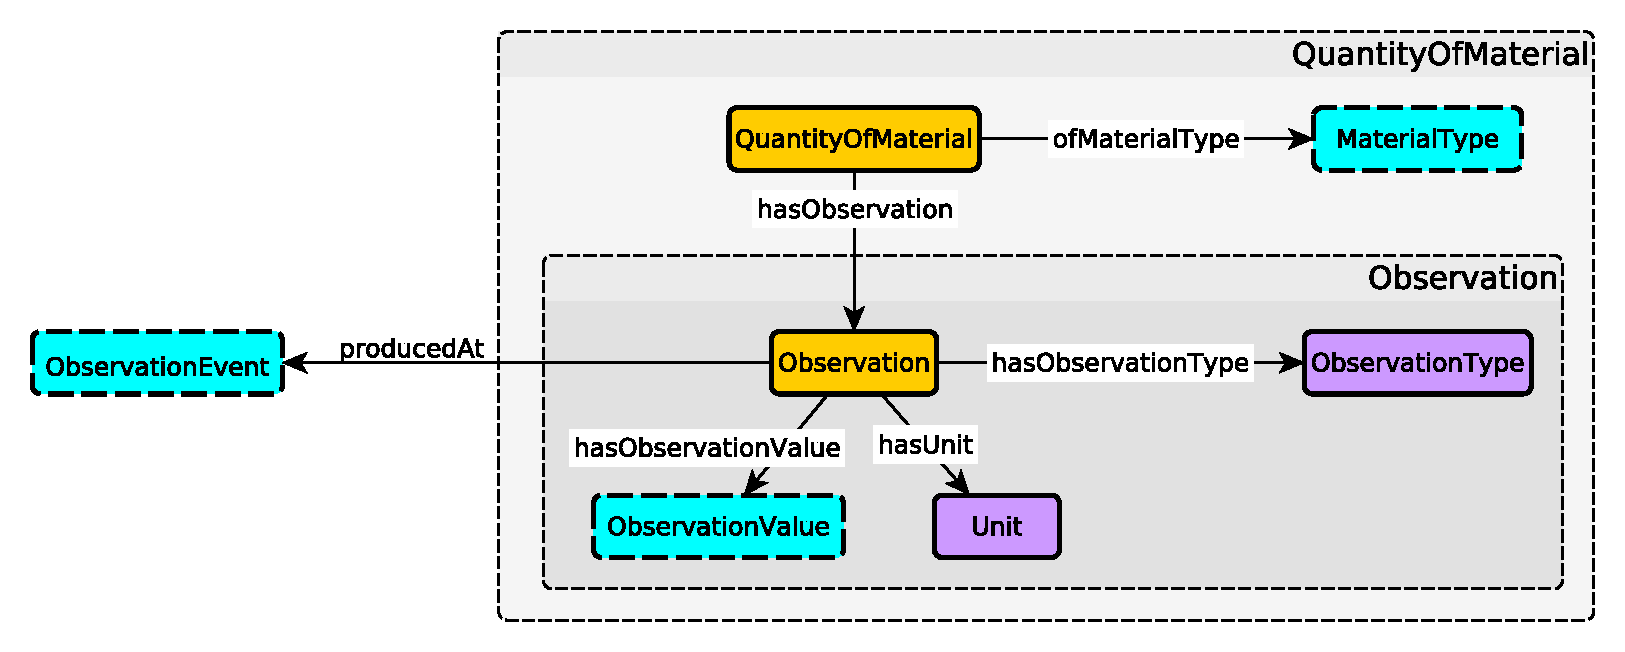
\includegraphics[width=.9\textwidth]{diagrams/quantity}
\end{center}
\caption{Schema Diagram for the Quantity of Material module}
\label{fig:quantity}
\end{figure}

\subsubsection*{Axioms:}
We use hMV for hasMeasurementValue.
\begin{align}
    \exists\textsf{ofMaterialType.MaterialType} &\sqsubseteq \textsf{QuantityOfMaterial}\\
    \textsf{QuantityOfMaterial} &\sqsubseteq \forall\textsf{ofMaterialType.MaterialType}\\
    \textsf{QuantityOfMaterial} &\sqsubseteq \exists\textsf{ofMaterialType.MaterialType}\\
    \textsf{QuantityOfMaterial} &\sqsubseteq \forall\textsf{hasMeasurement.Measurement}\\
    \exists\textsf{hasMeasurementType.MeasurementType} &\sqsubseteq \textsf{Measurement}\\ \textsf{Measurement} &\sqsubseteq \forall\textsf{hasMeasurementType.MeasurementType}\\ \textsf{Measurement} &\sqsubseteq \exists\textsf{hasMeasurementType.MeasurementType}\\
    \exists\textsf{hMV.MeasurementValue} &\sqsubseteq \textsf{Measurement}\\
    \textsf{Measurement} &\sqsubseteq \forall\textsf{hMV.MeasurementValue}\\
    \textsf{Measurement} &\sqsubseteq \exists\textsf{hMV.MeasurementValue}\\
    \textsf{Measurement} &\sqsubseteq \forall\textsf{hasUnit.Unit}\\
    \textsf{Measurement} &\sqsubseteq \exists\textsf{hasUnit.Unit}\\
    \textsf{Measurement} &\sqsubseteq \forall\textsf{producedAt.ObservationEvent}\\
    \textsf{Measurement} &\sqsubseteq \exists\textsf{producedAt.ObservationEvent}
\end{align}

\subsubsection*{Axiom Explanations:}
\begin{enumerate}
    \item Scoped Domain: The domain of \textsf{ofMaterialType} is \textsf{QuantityOfMaterial}, scoped by \textsf{MaterialType}.
    \item Scoped Range: The range of \textsf{ofMaterialType} is \textsf{MaterialType}, scoped by \textsf{QuantityOfMaterial}.
    \item Existential: \textsf{ofMaterialType}
    \item Scoped Range: The range of \textsf{hasMeasurement} is \textsf{Measurement}, scoped by \textsf{QuantityOfMaterial}.
    \item Scoped Domain: The domain of \textsf{hasMeasurementType} is \textsf{Measurement}, scoped by \textsf{MeasurementType}.
    \item Scoped Range: The range of \textsf{hasMeasurementType} is \textsf{Measurement}, scoped by \textsf{MeasurementType}.
    \item Existential: \textsf{hasMeasurementType}
    \item Scoped Domain: The domain of \textsf{hasMeasurementValue} is \textsf{Measurement}, scoped by \textsf{MeasurementValue}.
    \item Scoped Range: The range of \textsf{hasMeasurementValue} is \textsf{MeasurementValue}, scoped by \textsf{Measurement}.
    \item Existential: \textsf{hasMeasurementValue}
    \item Scoped Range: The range of \textsf{hasUnit} is \textsf{Unit}, scoped by \textsf{Measurement}.
    \item Existential: \textsf{hasUnit}
    \item Scoped Range: The range of \textsf{producedAt} is \textsf{ObservationEvent}, scoped by \textsf{Measurement}.
    \item Existential: \textsf{producedAt}
\end{enumerate}

\subsubsection*{Remarks:}
\begin{enumerate}
    \item A Measurement is a type of Observation. We use Observation for more general uses or qualitative assessments, such as smells. The same structure may be used for Measurement.
\end{enumerate}

%%%%%%%%%%%%%%%%%%%%%%%%%%%%%%%%%%%%%%%%%%%%%%%%%%%%%%%%
\section{Master Event}
\label{ssec:master}
%%%%%%%%%%%%%%%%%%%%%%%%%%%%
Master Event refers to an event model that can be understood as a generalized version of several of the relevant tracking events. While \emph{Master Event} by itself may not be of independent interest for the model, we include it here to show how the models for the different relevant tracking events relate to each other. After discussing this, we move to the more specific tracking event models, below. This module is a very significantly adapted version from the (very simple) Event pattern from \cite{MODL}. % \textbf{Scott suggestion: It addresses, e.g., the work done in the AgGateway CART project.}

\begin{figure}[tb]
\begin{center}
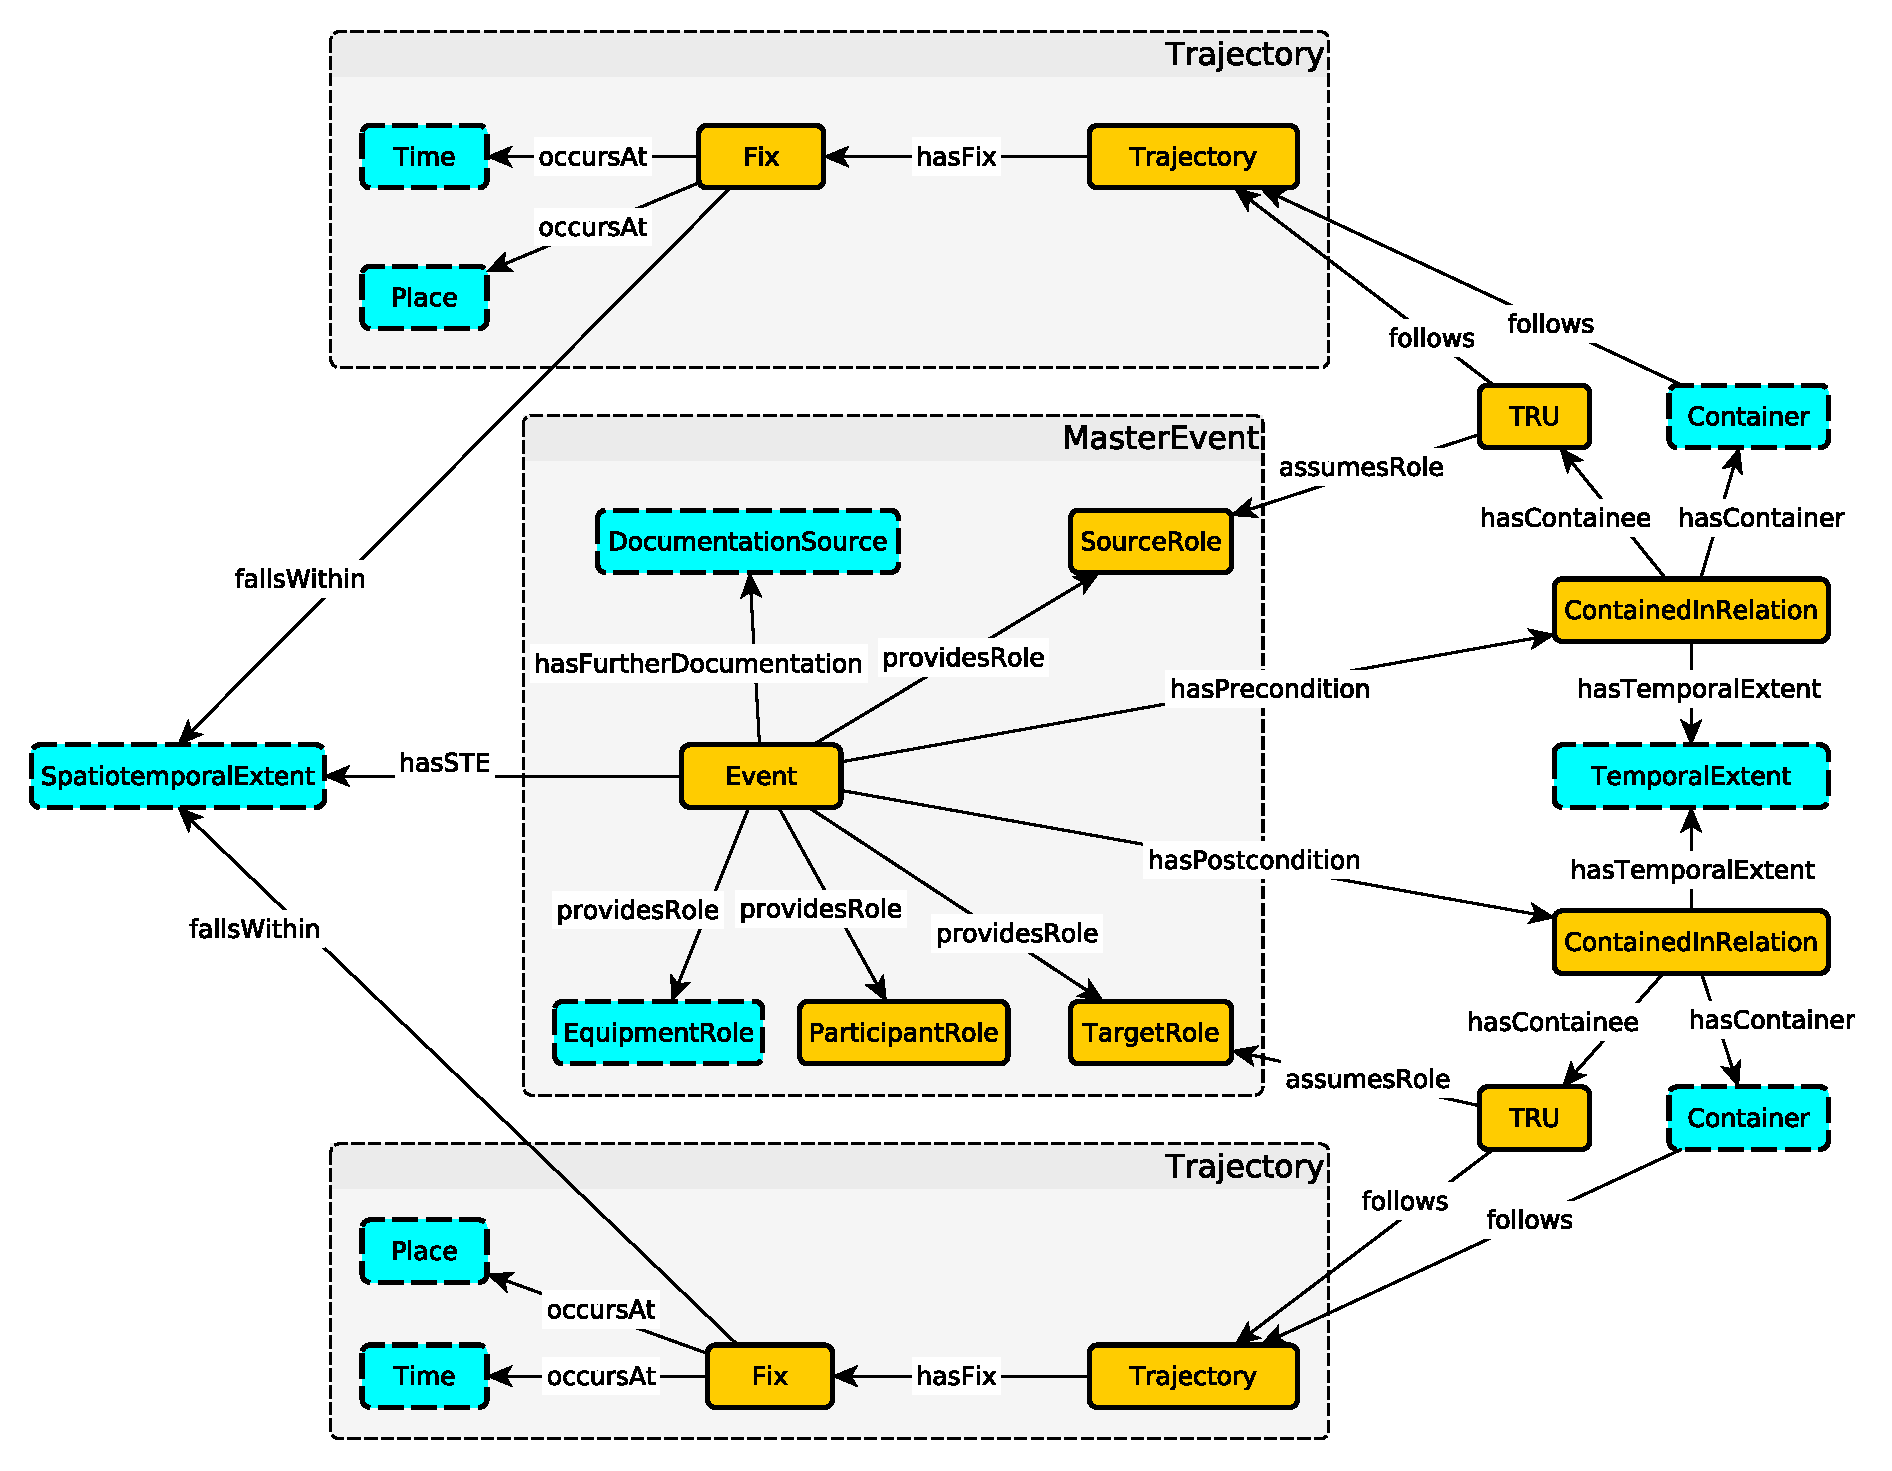
\includegraphics[width=\textwidth]{diagrams/master_event_no_duplicates}
\end{center}
\caption[Schema Diagram for the MasterEvent module (1)]{Schema Diagram for the MasterEvent module.}
\label{fig:masterEventnd}
\end{figure}

We give some explanations based on the schema diagram in Figure \ref{fig:masterEventnd}. The Event class can be found in the middle of the diagram. Events, in this conceptualization, happen in space and time (i.e., have spatiotemporal extents), and provide roles for participants (which may be agents or or other things relevant to the event under discussion). Participant roles are in particular provided for TRUs, and some TRUs may have \emph{source} roles, some may have \emph{target} roles. For example, content from source TRUs may get merged and re-divided, resulting in target TRUs at the end of the event. There may be multiple source and target TRUs (as depicted in the alternative diagram in Figure \ref{fig:masterEvent}). For some types of event, the ContainedInRelation (see the Container module) is relevant for the event, i.e. such a ContainedInRelation may be a constituent of a "pre" situation (meaning that it should be the case at the beginning of the event) and/or of a "post" situation (meaning that it should be the case at the end of the event).  TRUs, Containers, ContainedInRelations may persist throughout the event (remain unchanged), or may not. Other roles which may be relevant may be that of owner or custodian, used equipment, etc. Each type of critical tracking event will define corresponding relevant roles. We also provide a \emph{DocumentationSource} sub-module for information where further documentation for the event may be available.

\begin{figure}[tb]
\begin{center}
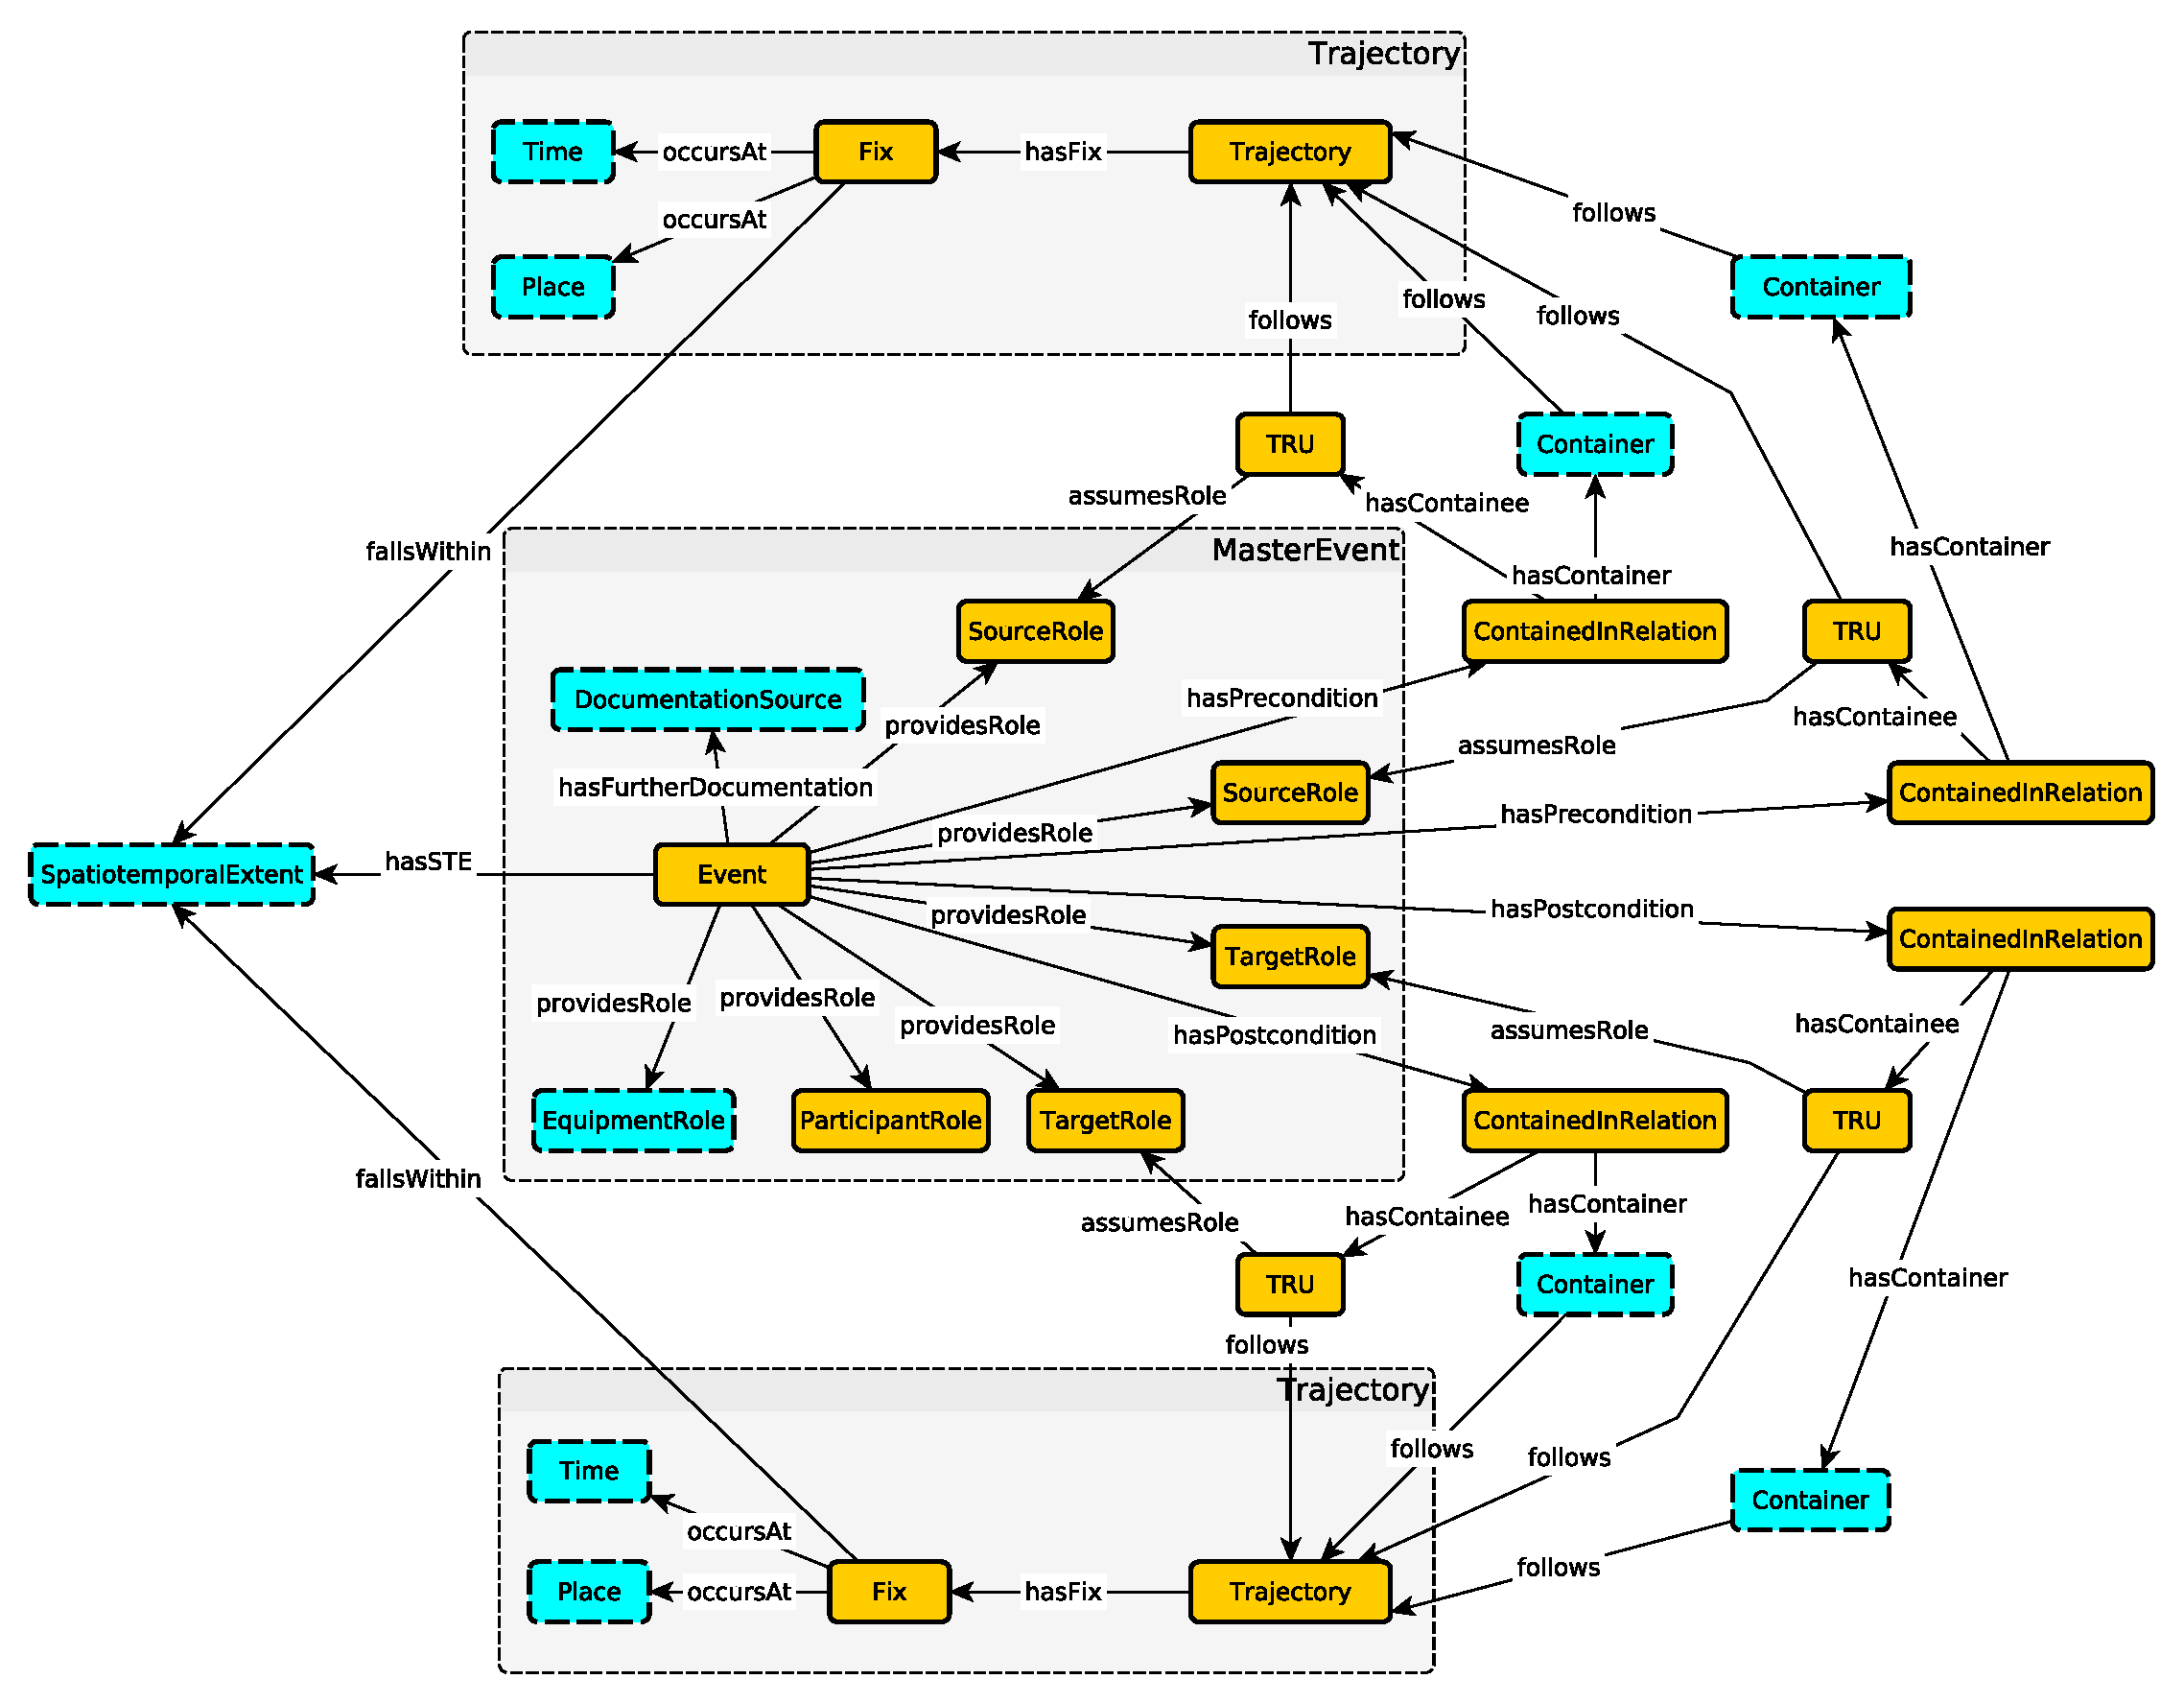
\includegraphics[width=\textwidth]{diagrams/master_event}
\end{center}
\caption[Alternative Schema Diagram for the MasterEvent module]{Schema Diagram for the MasterEvent module. This diagram deliberatly contains redundant elements to depict that there can be several source and target TRUs.}
\label{fig:masterEvent}
\end{figure}

\subsubsection*{Axioms:}
\begin{align}
    \top &\sqsubseteq \forall\textsf{hasSTE.SpatiotemporalExtent}\\
    \textsf{Event} &\sqsubseteq \exists\textsf{hasSTE.SpatiotemporalExtent}\\
    \textsf{Event} &\sqsubseteq \forall\textsf{providesRole.ParticipantRole}\\
    \textsf{ParticipantRole} &\sqsubseteq \mathord{\leq} 1 \textsf{providesRole}\mathord{^-}.\top\\
    \textsf{TRU} &\sqsubseteq \forall\textsf{assumesRole.ParticipantRole}\\
    \textsf{ParticipantRole} &\sqsubseteq \mathord{\leq} 1 \textsf{assumesRole}\mathord{^-}.\top\\
    \textsf{Event} &\sqsubseteq \forall\textsf{hasFurtherDocumentation.DocumentationSource} \\
    \textsf{SourceRole} &\sqsubseteq \textsf{ParticipantRole}\\
    \textsf{TargetRole} &\sqsubseteq \textsf{ParticipantRole}\\
    \textsf{EquipmentRole} &\sqsubseteq \textsf{ParticipantRole}\\
    \textsf{Event} &\sqsubseteq \mathord{\geq}0\textsf{hasPrecondition.ContainedInRelation}\\
    \textsf{Event} &\sqsubseteq \mathord{\geq}0\textsf{hasPostcondition.ContainedInRelation}
\end{align}

\subsubsection*{Axiom Explanations:}
\begin{enumerate}
    \item Range: The range of \textsf{hasSTE} is \textsf{SpatiotemporalExtent}.
    \item Existential: \textsf{hasSTE}
    \item Scoped Range: The range of \textsf{providesRole} is \textsf{ParticipantRole}, scoped by \textsf{Event}.
    \item Inverse Scoped Functionality: \textsf{providesRole}
    \item Scoped Range: The range of \textsf{assumesRole} is \textsf{Event}, scoped by \textsf{TRU}.
    \item Inverse Scoped Functionality: \textsf{assumesRole}
    \item Scoped Range: The range of \textsf{hasFurtherDocumentation} is \textsf{DocumentationSource}, scoped by \textsf{Event}.
    \item Subclass: Every \textsf{SourceRole} is a \textsf{ParticipantRole}.
    \item Subclass: Every \textsf{TargetRole} is a \textsf{ParticipantRole}.
    \item Subclass: Every \textsf{EquipmentRole} is a \textsf{ParticipantRole}.
    \item Structural Tautology: An \textsf{Event} may have a \textsf{ContainedInRelation} via \textsf{hasPrecondition}.
    \item Structural Tautology: An \textsf{Event} may have a \textsf{ContainedInRelation} via \textsf{hasPostcondition}.
\end{enumerate}

\subsubsection{Remarks:}
\begin{itemize}
    \item The following should be the case: If an Event E hasSTE S, then if a TRU assumes a role for this event, any container this TRU is currently contained in, should have a fix that fallsWithin S.
    \item \item Time (Trajectory module), TemporalScope (Container module) and SpatioTemporalExtent will have to be properly related when modeled.
\end{itemize}

%%%%%%%%%%%%%%%%%%%%%%%%%%%%%%%%%%%%%%%%%%%%%%%%%%%%%%%%
\subsection{Transfer Event}
\label{ssec:transfer}
%%%%%%%%%%%%%%%%%%%%%%%%%%%%
A Transfer Event happens when TRUs are combined, merged, split and/or moved into other containers. The diagram (and model) is essentially the Master Event model. 

\begin{figure}[tb]
\begin{center}
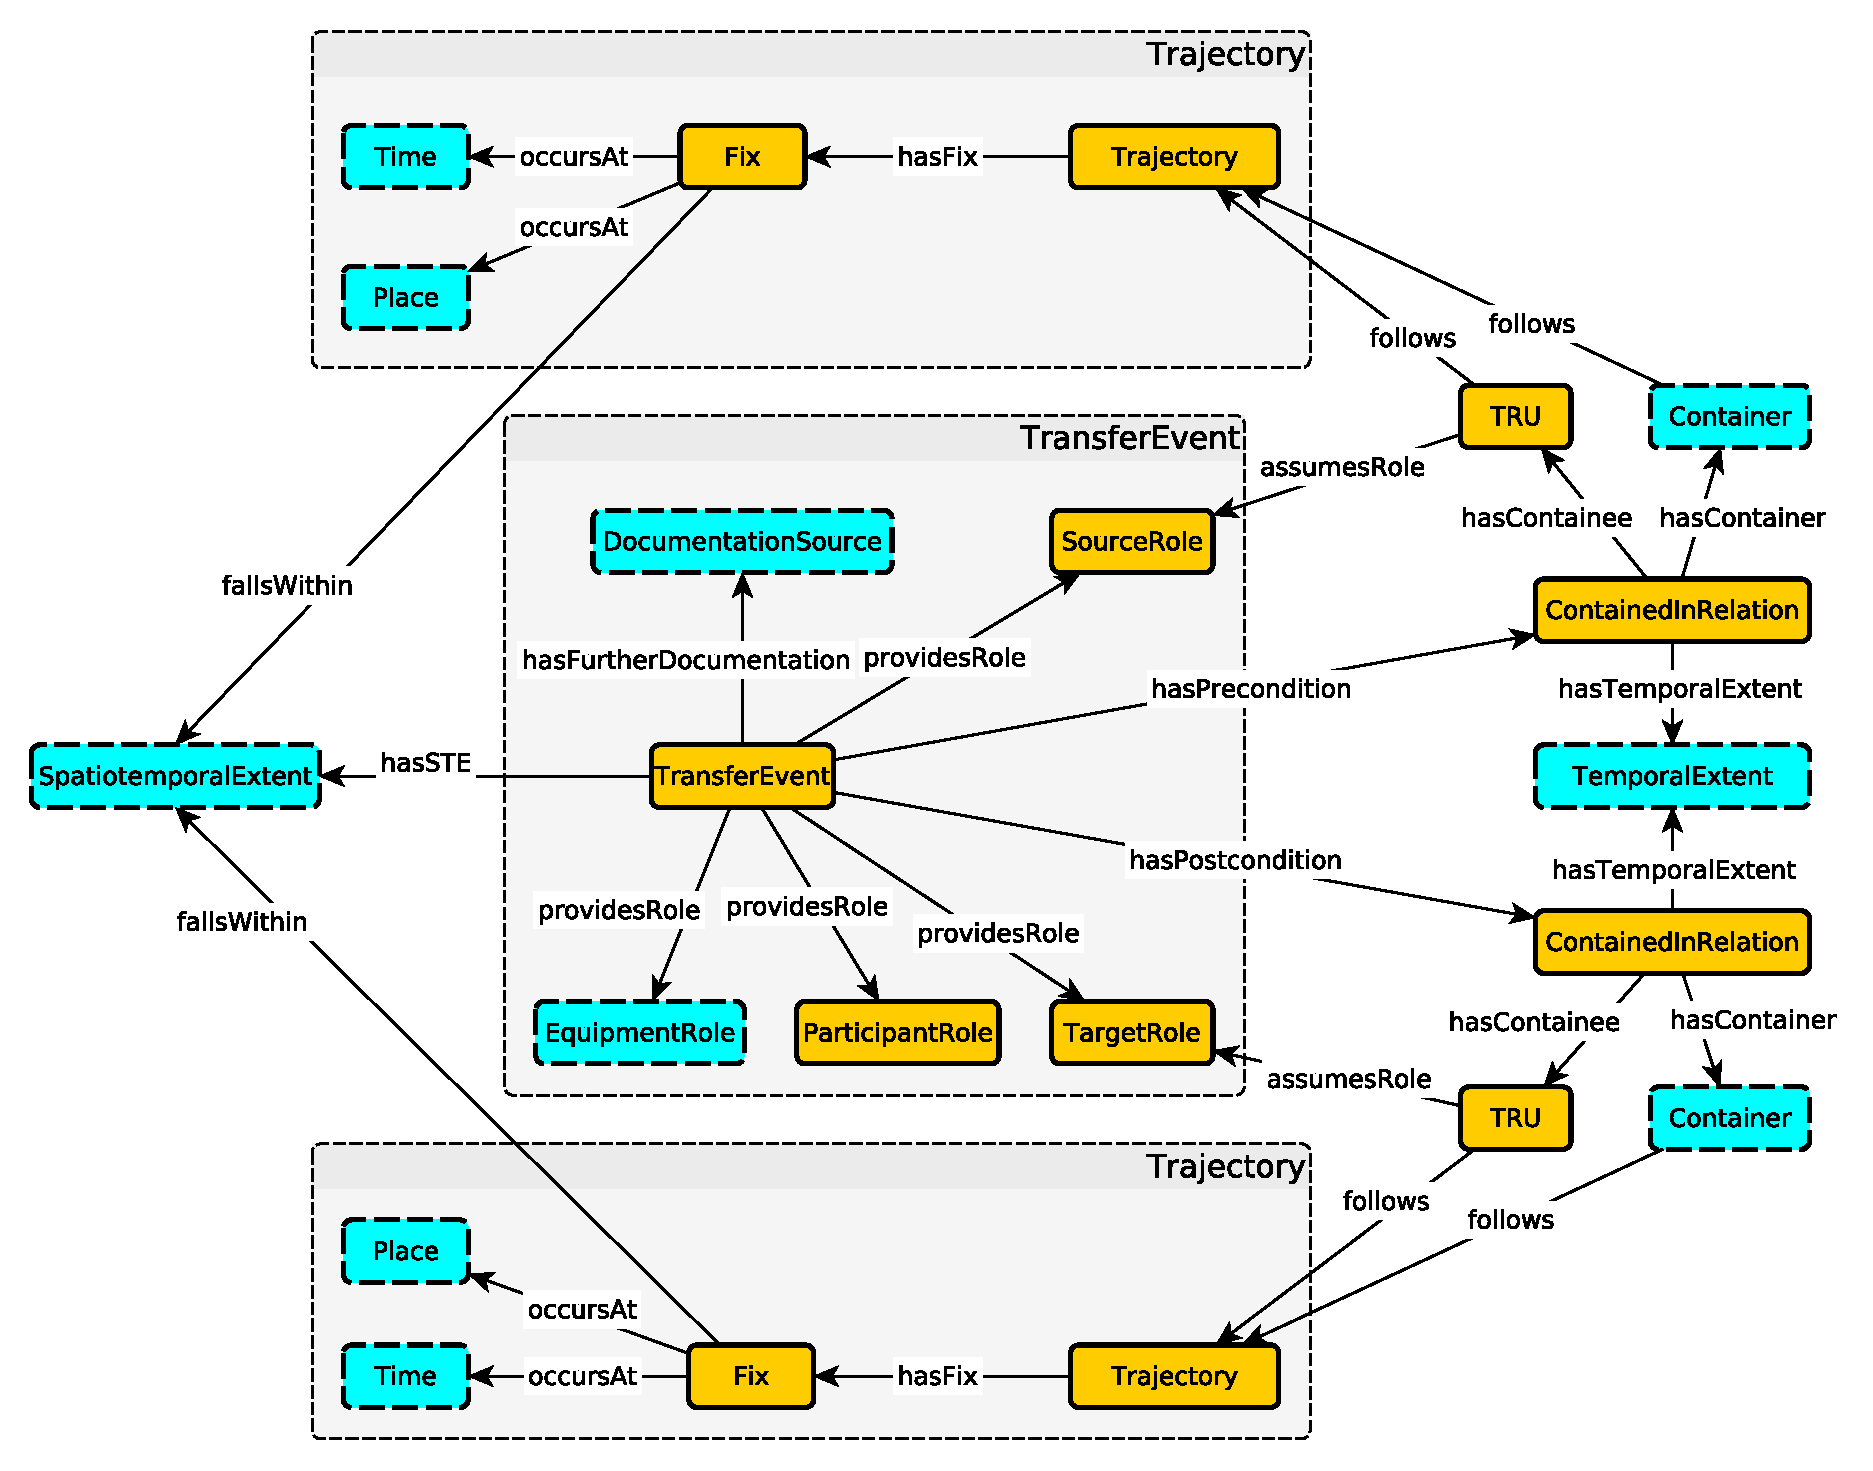
\includegraphics[width=\textwidth]{diagrams/transfer-event}
\end{center}
\caption{Schema Diagram for the TransferEvent module}
\label{fig:TransferEvent}
\end{figure}

\subsubsection*{Axioms:}
\begin{align}
    \top &\sqsubseteq \forall\textsf{hasSTE.SpatiotemporalExtent}\\
    \textsf{TransferEvent} &\sqsubseteq \exists\textsf{hasSTE.SpatiotemporalExtent}\\
    \textsf{TransferEvent} &\sqsubseteq \forall\textsf{providesRole.ParticipantRole}\\
    \textsf{ParticipantRole} &\sqsubseteq \mathord{\leq} 1 \textsf{providesRole}\mathord{^-}.\top\\
    \textsf{TRU} &\sqsubseteq \forall\textsf{assumesRole.ParticipantRole}\\
    \textsf{ParticipantRole} &\sqsubseteq \mathord{\leq} 1 \textsf{assumesRole}\mathord{^-}.\top\\
    \textsf{TransferEvent} &\sqsubseteq \forall\textsf{hasFurtherDocumentation.DocumentationSource} \\
    \textsf{SourceRole} &\sqsubseteq \textsf{ParticipantRole}\\
    \textsf{TargetRole} &\sqsubseteq \textsf{ParticipantRole}\\
    \textsf{TransferEvent} &\sqsubseteq \exists\textsf{providesRole}.(\textsf{SourceRole} \sqcap \exists \textsf{assumesRole}^-.\textsf{TRU})\\
    \textsf{TransferEvent} &\sqsubseteq \exists\textsf{providesRole}.(\textsf{TargetRole} \sqcap \exists \textsf{assumesRole}^-.\textsf{TRU})\\
    \textsf{TransferEvent} &\sqsubseteq \exists\textsf{hasPrecondition.ContainedInRelation}\\
    \textsf{TransferEvent} &\sqsubseteq \exists\textsf{hasPostcondition.ContainedInRelation}
\end{align}

\subsubsection*{Axiom Explanations:}
\begin{enumerate}
    \item Range: The range of \textsf{hasSTE} is \textsf{SpatiotemporalExtent}.
    \item Existential: \textsf{hasSTE}
    \item Scoped Range: The range of \textsf{providesRole} is \textsf{ParticipantRole}, scoped by \textsf{TransferEvent}.
    \item Inverse Scoped Functionality: \textsf{providesRole}
    \item Scoped Range: The range of \textsf{assumesRole} is \textsf{ParticipantRole}, scoped by \textsf{TransferEvent}.
    \item Inverse Scoped Functionality: \textsf{assumesRole}
    \item Scoped Range: The range of \textsf{hasFurtherDocumentation} is \textsf{DocumentationSource}, scoped by \textsf{TransferEvent}.
    \item Subclass: Every \textsf{SourceRole} is a \textsf{Participantrole}.
    \item Subclass: Every \textsf{TargetRole} is a \textsf{ParticipantRole}.
    \item existential and inverse functionality
    \item existential and inverse functionality
    \item Existential: \textsf{hasPrecondition}
    \item Existential: \textsf{hasPostcondition}
\end{enumerate}

\subsubsection{Remarks:}
\begin{itemize}
    \item The following should be the case: If an Event E hasSTE S, then if a TRU assumes a role for this event, any container this TRU is currently contained in, should have a fix that fallsWithin S.
\end{itemize}

%%%%%%%%%%%%%%%%%%%%%%%%%%%%%%%%%%%%%%%%%%%%%%%%%%%%%%%%
\subsection{Transformation Event}
\label{ssec:transformation}
%%%%%%%%%%%%%%%%%%%%%%%%%%%%
A Transformation Event occurs when there is a change of the nature of source TRU content that is different from the original form. E.g., grain may be transformed into flour. The transformation itself is understood to be a transformation activity. Other than that, this module is essentially the same as the MasterEvent module.

\begin{figure}[tb]
\begin{center}
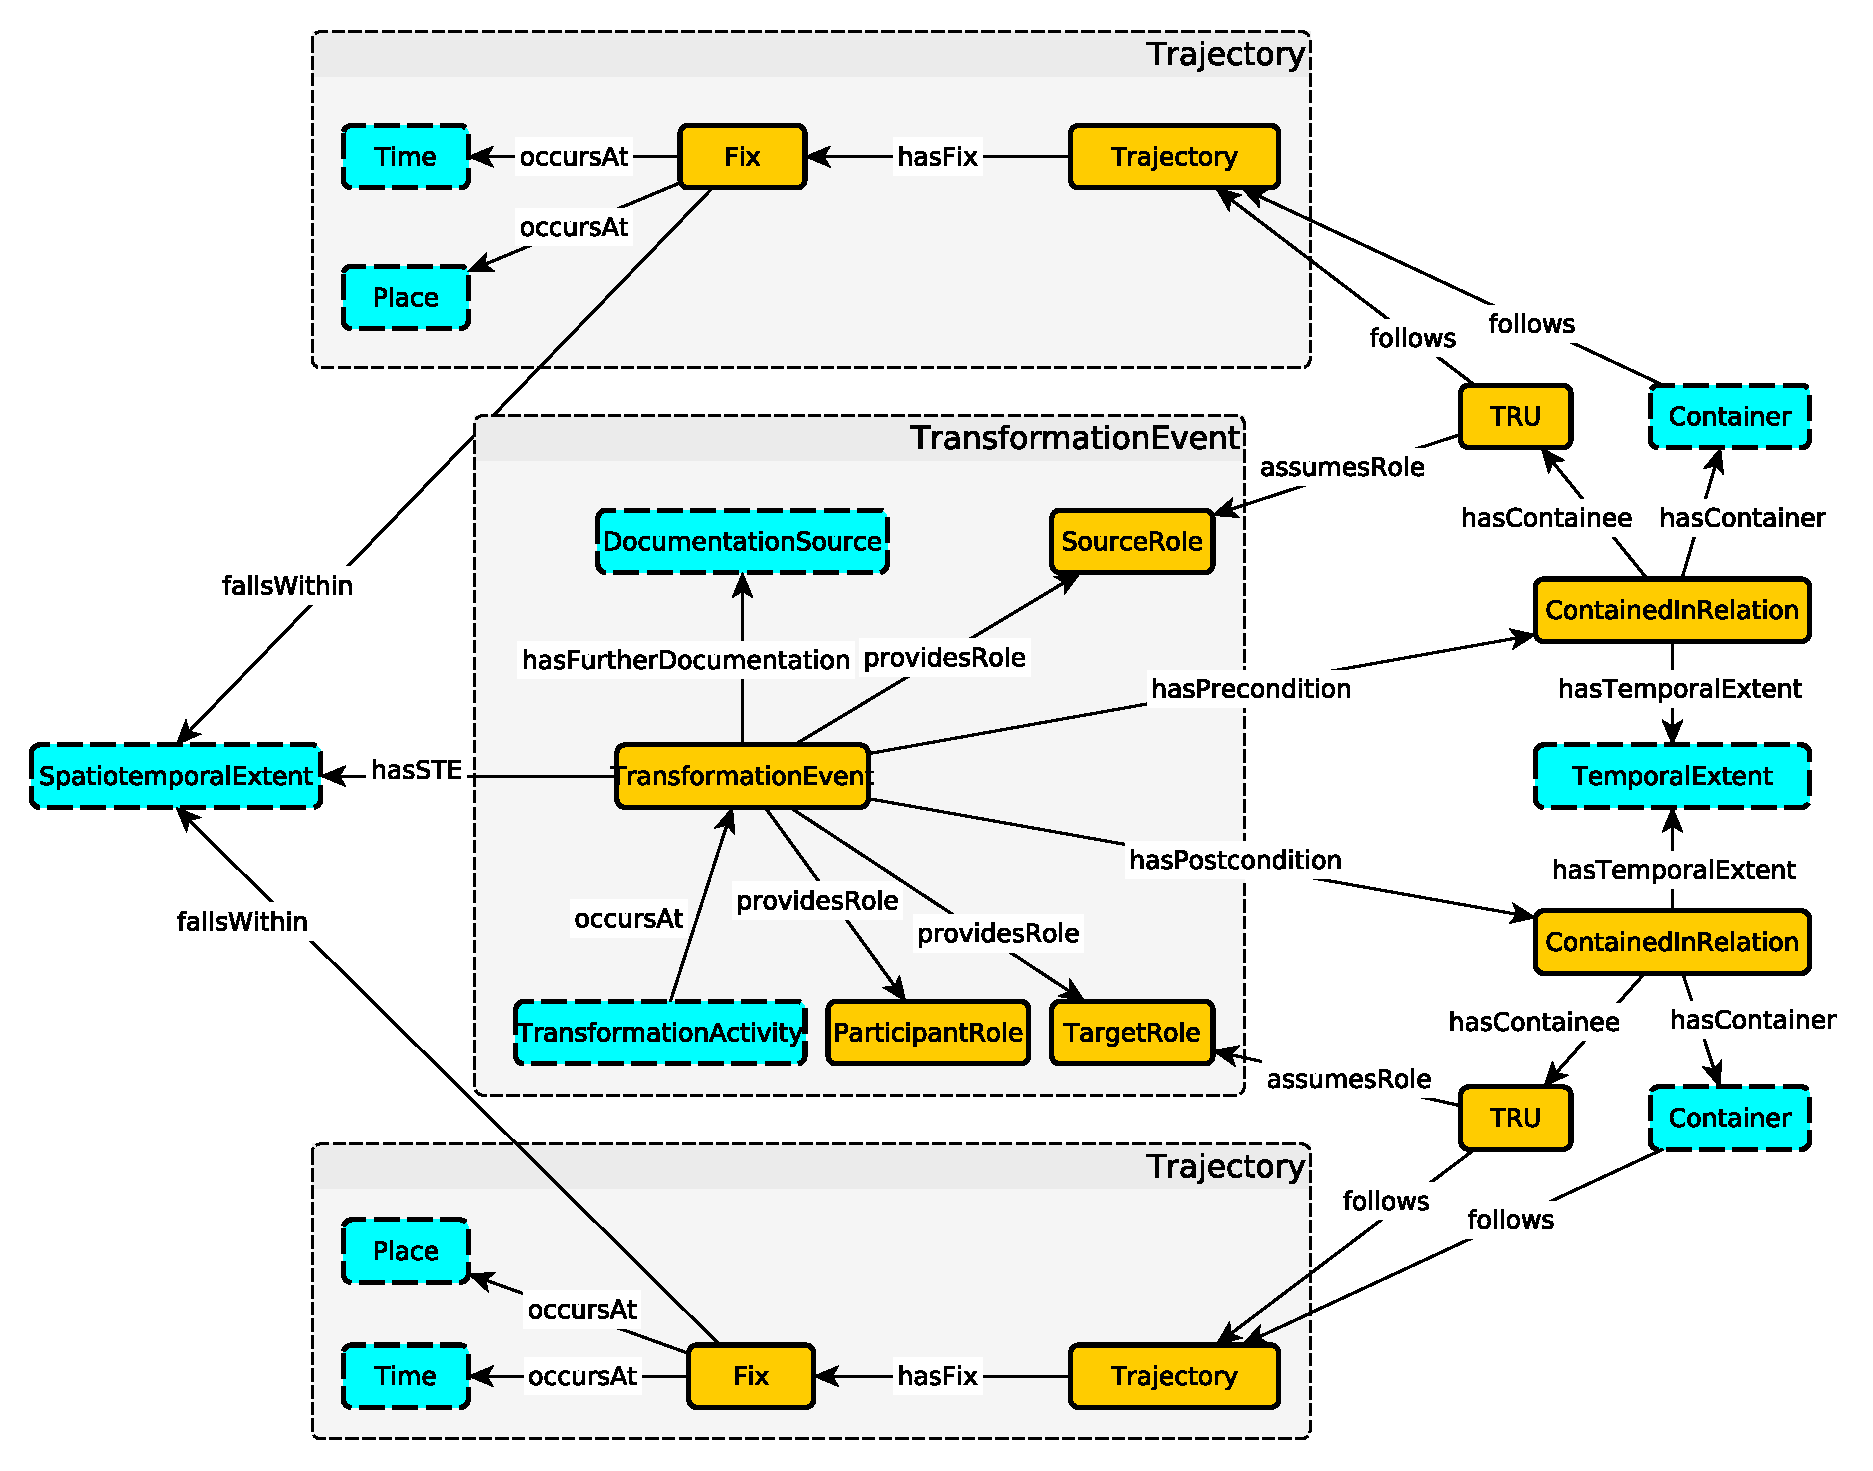
\includegraphics[width=.9\textwidth]{diagrams/transformation-event}
\end{center}
\caption{Schema Diagram for the TransformationEvent module}
\label{fig:TransformationEvent}
\end{figure}

\subsubsection*{Axioms:}
\begin{align}
\top &\sqsubseteq \forall\textsf{hasSTE.SpatiotemporalExtent}\\
\textsf{TransformationEvent} &\sqsubseteq \exists\textsf{hasSTE.SpatiotemporalExtent}\\
\textsf{TransformationEvent} &\sqsubseteq \forall\textsf{providesRole.SourceRole}\\
\textsf{ParticipantRole} &\sqsubseteq \mathord{\leq} 1 \textsf{providesRole}\mathord{^-}.\top\\
\textsf{TRU} &\sqsubseteq \forall\textsf{assumesRole.ParticipantRole}\\
\textsf{ParticipantRole} &\sqsubseteq \mathord{\leq} 1 \textsf{assumesRole}\mathord{^-}.\top\\
\textsf{TransformationEvent} &\sqsubseteq \forall\textsf{hasFurtherDocumentation.DocumentationSource} \\
\textsf{TransformationEvent} &\sqsubseteq \exists\textsf{occursAt}^-.\textsf{TransformationActivity}\\
\textsf{SourceRole} &\sqsubseteq \textsf{ParticipantRole}\\
\textsf{TargetRole} &\sqsubseteq \textsf{ParticipantRole}\\
\textsf{TransformationEvent} &\sqsubseteq \exists\textsf{providesRole}.(\textsf{SourceRole} \sqcap \exists \textsf{assumesRole}^-.\textsf{TRU})\\
\textsf{TransformationEvent} &\sqsubseteq \exists\textsf{providesRole}.(\textsf{TargetRole} \sqcap \exists \textsf{assumesRole}^-.\textsf{TRU})\\
\textsf{TransformationEvent} &\sqsubseteq \exists\textsf{hasPrecondition.ContainedInRelation}\\
\textsf{TransformationEvent} &\sqsubseteq \exists\textsf{hasPostcondition.ContainedInRelation}
\end{align}

\subsubsection*{Axiom Explanations:}
\begin{enumerate}
    \item Range: The range of \textsf{hasSTE} is \textsf{SpatiotemporalExtent}.
    \item Existential: \textsf{hasSTE}
    \item Scoped Range: The range of \textsf{providesRole} is \textsf{ParticipantRole}, scoped by \textsf{TransformationEvent}.
    \item Inverse Scoped Functionality: \textsf{providesRole}
    \item Scoped Range: The range of \textsf{assumesRole} is \textsf{ParticipantRole}, scoped by \textsf{TRU}.
    \item Inverse Scoped Functionality: \textsf{assumesRole}
    \item Scoped Range: The range of \textsf{hasFurtherDocumentation} is \textsf{DocumentationSource}, scoped by \textsf{TransformationEvent}.
    \item Inverse Existential: \textsf{occursAt}
    \item Subclass: Every \textsf{SourceRole} is a \textsf{ParticipantRole}.
    \item Subclass: Every \textsf{TargetRole} is a \textsf{ParticipantRole}.
    \item Existential and Inverse Functionality
    \item Existential and Inverse Functionality
    \item Existential: \textsf{hasPrecondition}
    \item Existential: \textsf{hasPostcondition}
\end{enumerate}

\subsubsection{Remarks:}
\begin{itemize}
    \item The following should be the case: If an Event E hasSTE S, then if a TRU assumes a role for this event, any container this TRU is currently contained in, should have a fix that fallsWithin S.
\end{itemize}

%%%%%%%%%%%%%%%%%%%%%%%%%%%%%%%%%%%%%%%%%%%%%%%%%%%%%%%%
\subsection{Custody Change Event}
\label{ssec:custody}
%%%%%%%%%%%%%%%%%%%%%%%%%%%%
A Custody Change Event occurs when the custodian of a TRU and/or Container changes. For this event, the classes SourceCustodianRole and TargetCustodianRole, as subclasses of ParticipantRole, are central. The diagram in Figure \ref{fig:CustodyChangeEvent} avoids the visual duplication of nodes used in the previous event diagrams.

\begin{figure}[tb]
\begin{center}
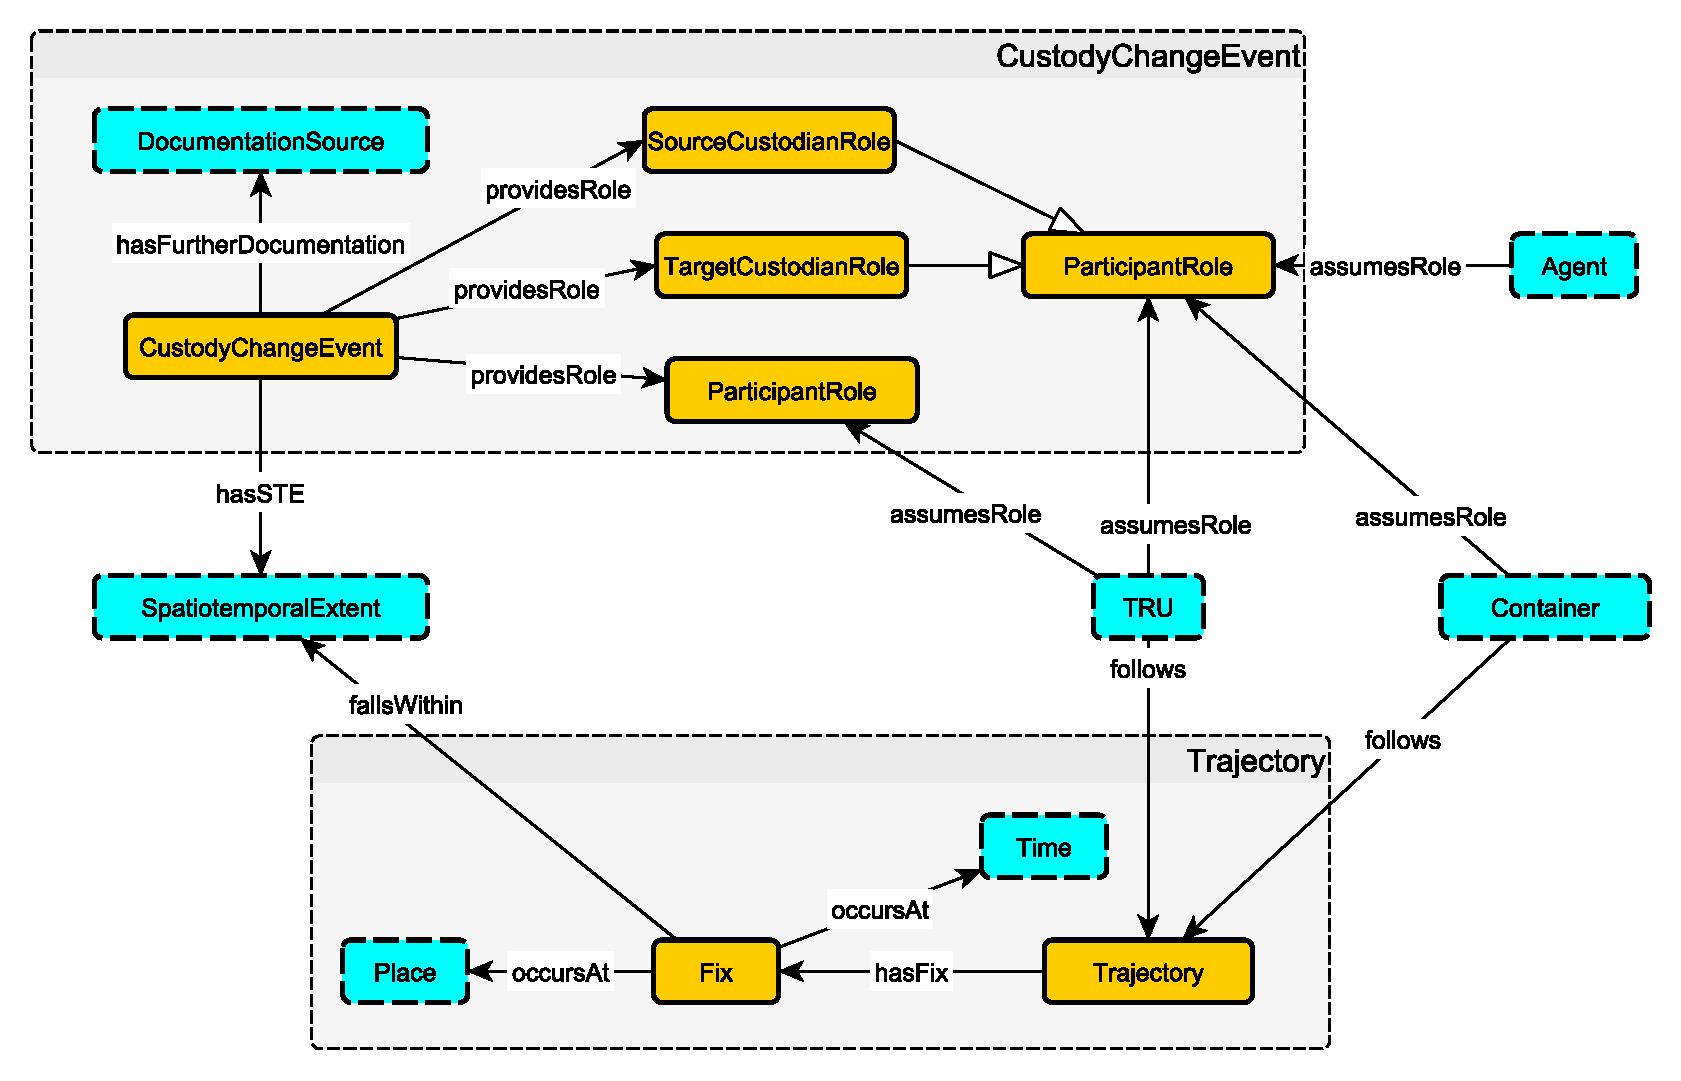
\includegraphics[width=.9\textwidth]{diagrams/custody-change_event}
\end{center}
\caption{Schema Diagram for the CustodyChangeEvent module}
\label{fig:CustodyChangeEvent}
\end{figure}

\subsubsection*{Axioms:}
\begin{align}
\top &\sqsubseteq \forall\textsf{hasSTE.SpatiotemporalExtent}\\
\textsf{CustodyChangeEvent} &\sqsubseteq \exists\textsf{hasSTE.}\\
\textsf{CustodyChangeEvent} &\sqsubseteq \forall\textsf{providesRole.ParticipantRole}\\
\textsf{ParticipantRole} &\sqsubseteq \mathord{\leq} 1 \textsf{providesRole}\mathord{^-}.\top\\
\textsf{TRU} &\sqsubseteq \forall\textsf{assumesRole.ParticipantRole}\\
\textsf{ParticipantRole} &\sqsubseteq \mathord{\leq} 1 \textsf{assumesRole}\mathord{^-}.\top\\
\textsf{CustodyChangeEvent} &\sqsubseteq \forall\textsf{hasFurtherDocumentation.DocumentationSource} \\
\textsf{SourceCustodianRole} &\sqsubseteq \textsf{ParticipantRole}\\
\textsf{TargetCustodianRole} &\sqsubseteq \textsf{ParticipantRole}\\
\textsf{CustodyChangeEvent} &\sqsubseteq \exists\textsf{providesRole}.(\textsf{SourceCustodianRole} \sqcap \exists \textsf{assumesRole}^-.\textsf{Agent})\\
\textsf{CustodyChangeEvent} &\sqsubseteq \exists\textsf{providesRole}.(\textsf{TargetCustodianRole} \sqcap \exists \textsf{assumesRole}^-.\textsf{Agent})\\
\textsf{CustodyChangeEvent} &\sqsubseteq \mathord{\lte}1\textsf{providesRole.SourceCustodianRole}\\
\textsf{CustodyChangeEvent} &\sqsubseteq \mathord{\lte}1\textsf{providesRole.TargetCustodianRole} 
\end{align}

\subsubsection*{Axiom Explanations:}
\begin{enumerate}
    \item Range: The range of \textsf{hasSTE} is \textsf{SpatiotemporalExtent}.
    \item Existential: \textsf{hasSTE}
    \item Scoped Range: The range of \textsf{providesRole} is \textsf{ParticipantRole}, scoped by \textsf{CustodyChangeEvent}.
    \item Inverse Scoped Functionality: \textsf{providesRole}
    \item Scoped Range: The range of \textsf{assumesRole} is \textsf{ParticipantRole}, scoped by \textsf{TRU}.
    \item Inverse Scoped Functionality: \textsf{assumesRole}
    \item Scoped Range: The range of \textsf{hasFurtherDocumentation} is \textsf{DocumentationSource}, scoped by \textsf{CustodyChangeEvent}.
    \item Subclass: Every \textsf{SourceCustodianRole} is a \textsf{ParticipantRole}.
    \item Subclass: Every \textsf{TargetCustodianRole} is a \textsf{ParticipantRole}.
    \item Existential and Inverse Functionality
    \item Existential and Inverse Functionality
    \item Functionality
    \item Functionality
\end{enumerate}

\subsubsection{Remarks:}
\begin{itemize}
    \item The following should be the case: If an Event E hasSTE S, then if a TRU assumes a role for this event, any container this TRU is currently contained in, should have a fix that fallsWithin S.
    \item ContainedInRelations are not depicted as they are considered unchanged by this type of Event.
\end{itemize}

%%%%%%%%%%%%%%%%%%%%%%%%%%%%%%%%%%%%%%%%%%%%%%%%%%%%%%%%
\subsection{Ownership Change Event}
\label{ssec:owner}
%%%%%%%%%%%%%%%%%%%%%%%%%%%%
An Ownership Change Event occurs when the owner of a TRU and/or Container changes. For this event, the classes SourceOwnerRole and TargetOwnerRole, as subclasses of ParticipantRole, are central. The diagram in Figure \ref{fig:OwnerChangeEvent} avoids the visual duplication of nodes used in the previous event diagrams.

\begin{figure}[tb]
\begin{center}
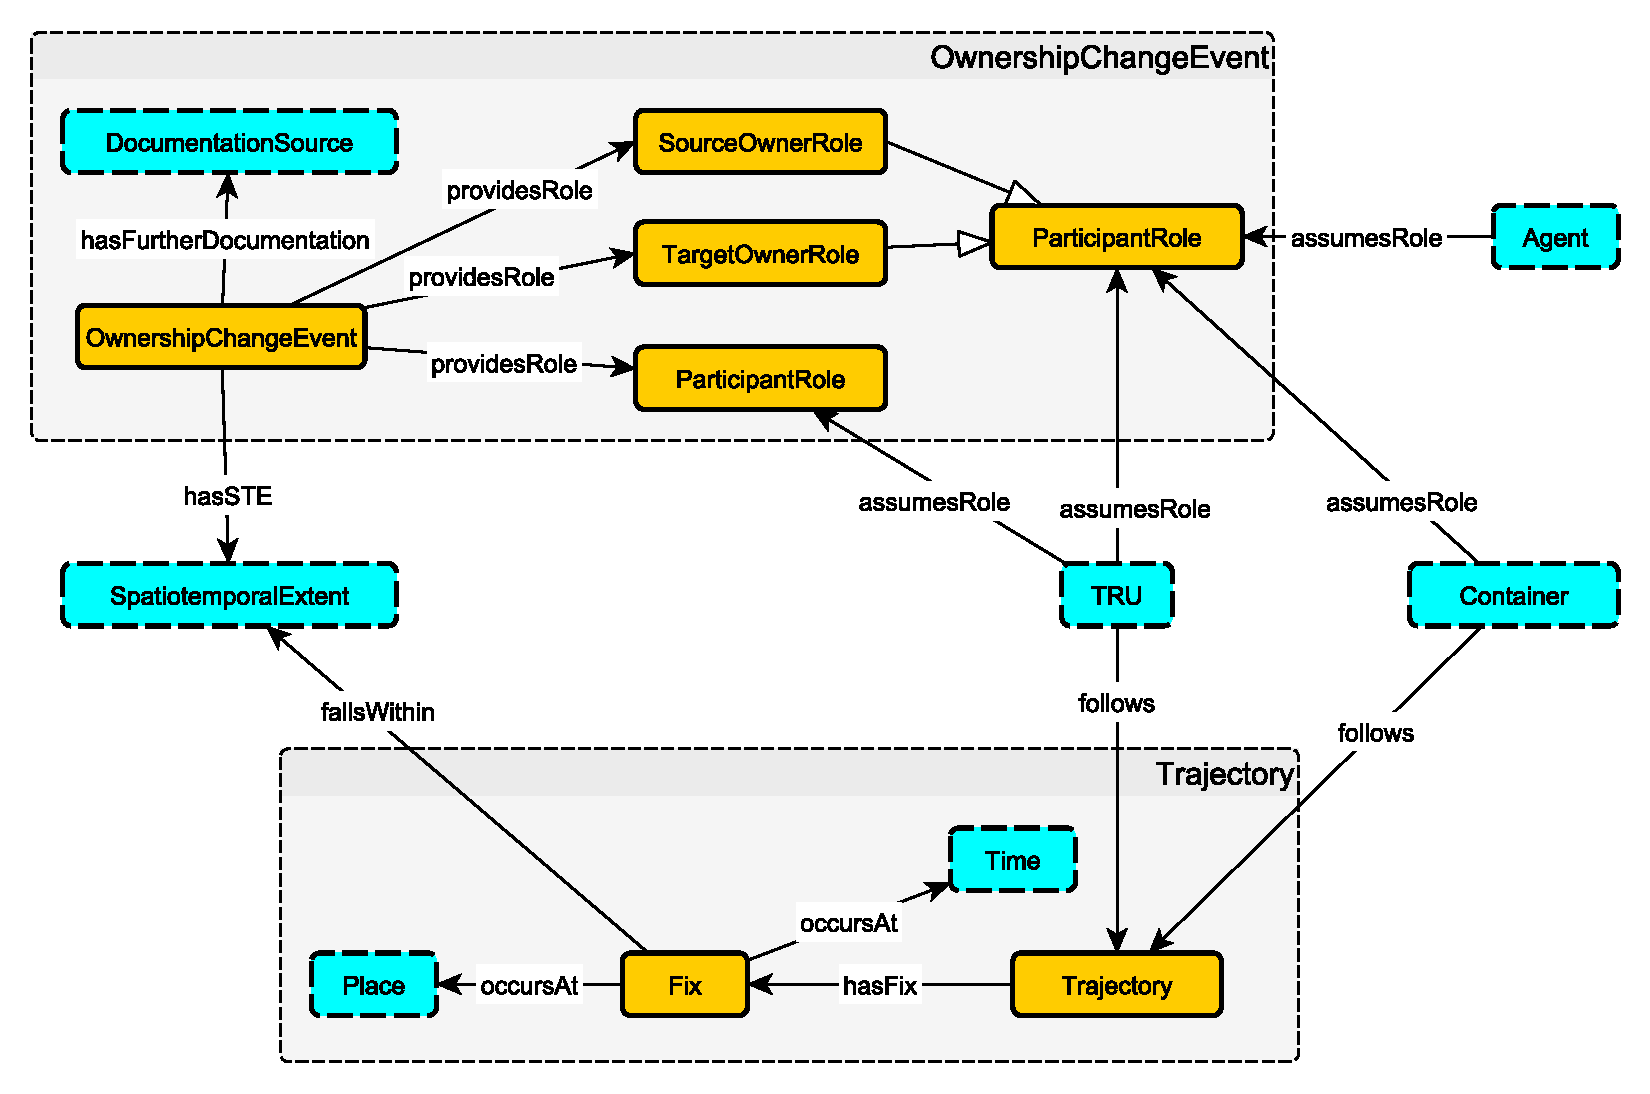
\includegraphics[width=.9\textwidth]{diagrams/owner-change_event}
\end{center}
\caption{Schema Diagram for the OwnerChangeEvent module}
\label{fig:OwnerChangeEvent}
\end{figure}

\subsubsection*{Axioms:}
\begin{align}
    \top &\sqsubseteq \forall\textsf{hasSTE.SpatiotemporalExtent}\\
    \textsf{OwnerChangeEvent} &\sqsubseteq \exists\textsf{hasSTE.SpatiotemporalExtent}\\
    \textsf{OwnerChangeEvent} &\sqsubseteq \forall\textsf{providesRole.ParticipantRole}\\
    \textsf{ParticipantRole} &\sqsubseteq \mathord{\leq}1 \textsf{providesRole}\mathord{^-}.\top\\
    \textsf{TRU} &\sqsubseteq \forall\textsf{assumesRole.ParticipantRole}\\
    \textsf{ParticipantRole} &\sqsubseteq \mathord{\leq} 1 \textsf{assumesRole}\mathord{^-}.\top\\
    \textsf{OwnerChangeEvent} &\sqsubseteq \forall\textsf{hasFurtherDocumentation.DocumentationSource} \\
    \textsf{SourceOwnerRole} &\sqsubseteq \textsf{ParticipantRole}\\
    \textsf{TargetOwnerRole} &\sqsubseteq \textsf{ParticipantRole}\\
    \textsf{OwnerChangeEvent} &\sqsubseteq \exists\textsf{providesRole}.(\textsf{SourceOwnerRole} \sqcap \exists \textsf{assumesRole}^-.\textsf{Agent})\\
    \textsf{OwnerChangeEvent} &\sqsubseteq \exists\textsf{providesRole}.(\textsf{TargetOwnerRole} \sqcap \exists \textsf{assumesRole}^-.\textsf{Agent})\\
    \textsf{OwnerChangeEvent} &\sqsubseteq \mathord{\leq}1\textsf{providesRole.SourceOwnerRole}\\
    \textsf{OwnerChangeEvent} &\sqsubseteq \mathord{\leq}1\textsf{providesRole.TargetOwnerRole} 
\end{align}

\subsubsection*{Axiom Explanations:}
\begin{enumerate}
    \item Range: The range of \textsf{hasSTE} is \textsf{SpatiotemporalExtent}.
    \item Existential: \textsf{hasSTE}
    \item Scoped Range: The range of \textsf{providesRole} is \textsf{ParticipantRole}, scoped by \textsf{OwnershipChangeEvent}.
    \item Inverse Scoped Functionality: \textsf{providesRole}
    \item Scoped Range: The range of \textsf{assumesRole} is \textsf{ParticipantRole}, scoped by \textsf{TRU}.
    \item Inverse Scoped Functionality: \textsf{assumesRole}
    \item Scoped Range: The range of \textsf{hasFurtherDocumentation} is \textsf{DocumentationSource}, scoped by \textsf{OwnerChangeEvent}.
    \item Subclass: Every \textsf{SourceOwnerRole} is a \textsf{ParticipantRole}.
    \item Subclass: Every \textsf{TargetOwnerRole} is a \textsf{ParticipantRole}.
    \item Existential and Inverse Functionality
    \item Existential and Inverse Functionality
    \item Functionality 
    \item Functionality
\end{enumerate}

\subsubsection{Remarks:}
\begin{itemize}
    \item The following should be the case: If an Event E hasSTE S, then if a TRU assumes a role for this event, any container this TRU is currently contained in, should have a fix that fallsWithin S.
    \item ContainedInRelations are not depicted as they are considered unchanged by this type of Event.
\end{itemize}

%%%%%%%%%%%%%%%%%%%%%%%%%%%%%%%%%%%%%%%%%%%%%%%%%%%%%%%%
\subsection{Transport Event}
\label{ssec:ocrec}
%%%%%%%%%%%%%%%%%%%%%%%%%%%%
A Transport Event occurs when a TRU is moved (being shipped) from one location to another location over an elapsed period of time. A container containing this TRU moves a long a trajectory which is entirely within the spatiotemporal extent of the Transport Event. It is important to note that ObservationEvents may happen concurrently, e.g. for measuring temperatures. 

\begin{figure}[tb]
\begin{center}
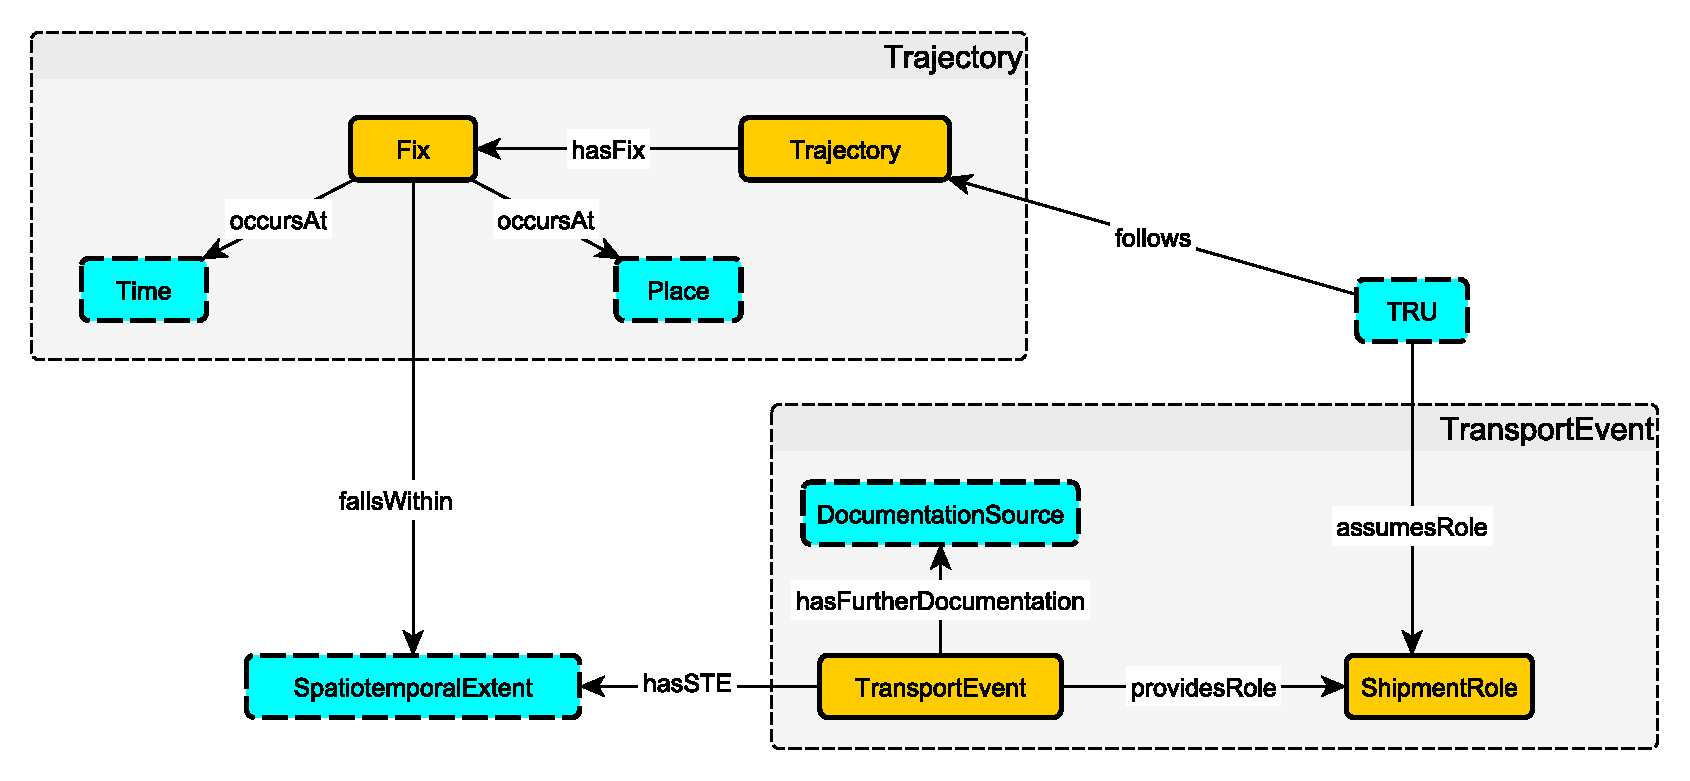
\includegraphics[width=.9\textwidth]{diagrams/transport-event}
\end{center}
\caption{Schema Diagram for the TransportEvent module}
\label{fig:TransportEvent}
\end{figure}

\subsubsection*{Axioms:}
\begin{align}
    \top &\sqsubseteq \forall\textsf{hasSTE.SpatiotemporalExtent}\\
    \textsf{TransportEvent} &\sqsubseteq \exists\textsf{hasSTE.SpatiotemporalExtent}\\
    \textsf{TransportEvent} &\sqsubseteq \forall\textsf{providesRole.ParticipantRole}\\
    \textsf{ParticipantRole} &\sqsubseteq \mathord{\leq} 1 \textsf{providesRole}\mathord{^-}.\top\\
    \textsf{TRU} &\sqsubseteq \forall\textsf{assumesRole.ParticipantRole}\\
    \textsf{ParticipantRole} &\sqsubseteq \mathord{\leq} 1 \textsf{assumesRole}\mathord{^-}.\top\\
    \textsf{TransportEvent} &\sqsubseteq \forall\textsf{hasFurtherDocumentation.DocumentationSource} \\
    \textsf{ShipmentRole} &\sqsubseteq \textsf{ParticipantRole}\\
    \textsf{TransportEvent} &\sqsubseteq \exists\textsf{providesRole}.(\textsf{ShipmentRole} \sqcap \exists \textsf{assumesRole}^-.\textsf{TRU})
\end{align}

\subsubsection*{Axiom Explanations:}
\begin{enumerate}
    \item Range: The range of \textsf{hasSTE} is \textsf{SpatiotemporalExtent}.
    \item Existential: \textsf{hasSTE}
    \item Scoped Range: The range of \textsf{providesRole} is \textsf{ParticipantRole}, scoped by \textsf{TransportEvent}.
    \item Inverse Scoped Functionality: \textsf{providesRole}
    \item Scoped Range: The range of \textsf{assumesRole} is \textsf{ParticipantRole}, scoped by \textsf{TRU}.
    \item Inverse Scoped Functionality: \textsf{assumesRole}
    \item Scoped Range: The range of \textsf{hasFurtherDocumentation} is \textsf{DocumentSource}, scoped by \textsf{TransportEvent}.
    \item Subclass: Every \textsf{TransportEvent} is a \textsf{ParticipantRole}.
    \item existential and inverse functionality
\end{enumerate}

\subsubsection{Remarks:}
\begin{itemize}
    \item The following should be the case: If an Event E hasSTE S, then if a TRU assumes a role for this event, any container this TRU is currently contained in, should have a fix that fallsWithin S.
    \item ContainedInRelations are not depicted as they are considered unchanged by this type of Event.
\end{itemize}

%%%%%%%%%%%%%%%%%%%%%%%%%%%%%%%%%%%%%%%%%%%%%%%%%%%%%%%%
\subsection{Observation Event}
\label{ssec:observation}
%%%%%%%%%%%%%%%%%%%%%%%%%%%%
An Observation Event occurs when a Measurement or other result on a TRU is captured at a specific point in time. 

\begin{figure}[tb]
\begin{center}
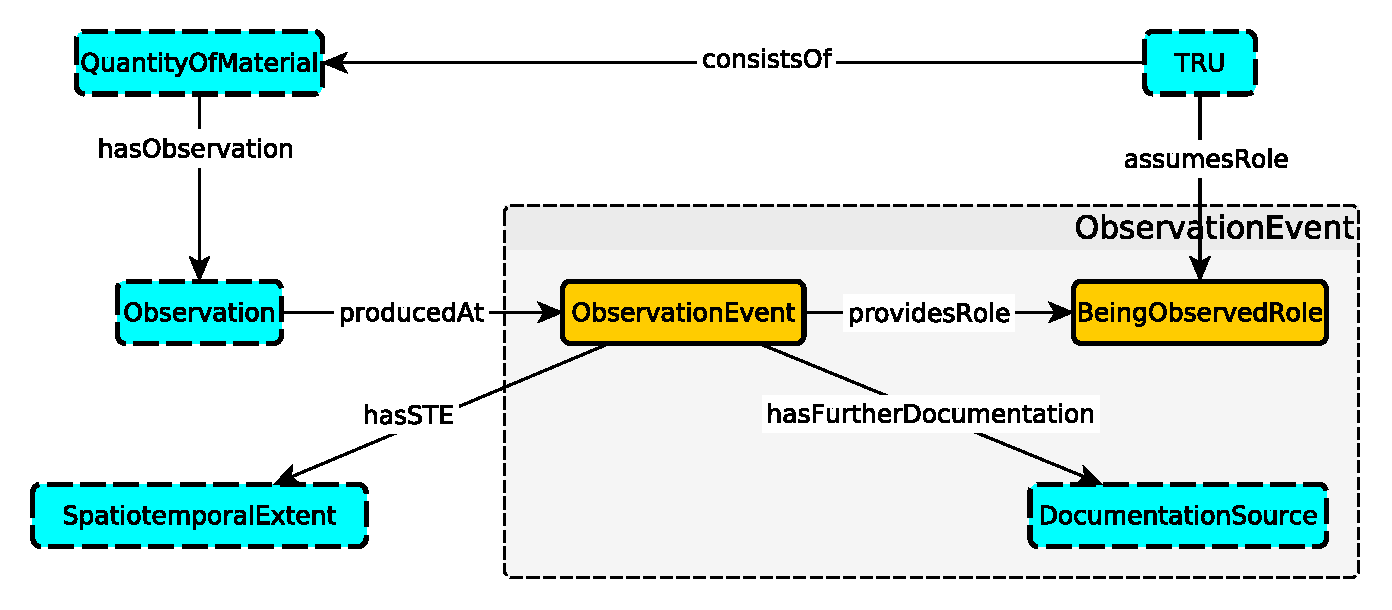
\includegraphics[width=.8\textwidth]{diagrams/observation_event}
\end{center}
\caption{Schema Diagram for the ObservationEvent module}
\label{fig:ObservationEvent}
\end{figure}

\subsubsection*{Axioms:}
\begin{align}
    \top &\sqsubseteq \forall\textsf{hasSTE.SpatiotemporalExtent}\\
    \textsf{ObservationEvent} &\sqsubseteq \exists\textsf{hasSTE.SpatiotemporalExtent}\\
    \textsf{ObservationEvent} &\sqsubseteq \forall\textsf{providesRole.ParticipantRole}\\
    \textsf{ParticipantRole} &\sqsubseteq \mathord{\leq} 1 \textsf{providesRole}\mathord{^-}.\top\\
    \textsf{TRU} &\sqsubseteq \forall\textsf{assumesRole.ParticipantRole}\\
    \textsf{ParticipantRole} &\sqsubseteq \mathord{\leq} 1 \textsf{assumesRole}\mathord{^-}.\top\\
    \textsf{ObservationEvent} &\sqsubseteq \forall\textsf{hasFurtherDocumentation.DocumentationSource} \\
    \textsf{BeingObservedRole} &\sqsubseteq \textsf{ParticipantRole}\\
    \textsf{Measurement} &\sqsubseteq \forall\textsf{producedAt.ObservationEvent}\\
    \textsf{ObservationEvent} &\sqsubseteq \exists\textsf{producedAt}^-.\textsf{Measurement}\\
    \textsf{ObservationEvent} &\sqsubseteq \exists\textsf{providesRole}.(\textsf{BeingObservedRole} \sqcap \exists \textsf{assumesRole}^-.\textsf{TRU})\\
    \textsf{TRU}(x) \wedge \textsf{consistsOf}(x,y) &\wedge \textsf{QuantityOfMaterial}(y) \wedge \textsf{hasMeasurement}(y,z)\nonumber\\ \phantom{k} \wedge \textsf{Measurement}(z) &\wedge \textsf{producedAt}(z,w) \wedge \textsf{ObservationEvent}(w)\nonumber\\ &\to \exists v (\textsf{BeingObservedRole}(v) \wedge \textsf{providesRole}(w,v)\nonumber\\ &\phantom{\wedge} \phantom{xxxxxxxxxxxxx} \wedge \textsf{assumesRole}(x,v))
\end{align}

\subsubsection*{Axiom Explanations:}
\begin{enumerate}
    \item Range: The range of \textsf{hasSTE} is \textsf{SpatiotemporalExtent}.
    \item Existential: \textsf{hasSTE}
    \item Scoped Range: The range of \textsf{providesRole} is \textsf{ParticipantRole}, scoped by \textsf{ObservationEvent}.
    \item Inverse Scoped Functionality: \textsf{providesRole}
    \item Scoped Range: The range of \textsf{assumesRole} is \textsf{ParticipantRole}, scoped by \textsf{TRU}.
    \item Inverse Scoped Functionality: \textsf{assumesRole}
    \item Scoped Range: The range of \textsf{hasFurtherDocumentation} is \textsf{DocumentationSource}, scoped by \textsf{ObservationEvent}.
    \item Subclass: Every \textsf{BeingObservedRole} is a \textsf{ParticipantRole}.
    \item Scoped Range: The range of \textsf{producedAt} is \textsf{ObservationEvent}, scoped by \textsf{Measurement}.
    \item Inverse Existential: \textsf{producedAt}
    \item existential and inverse functionality
    \item existential rule
\end{enumerate}

\subsubsection{Remarks:}
\begin{itemize}
    \item The following should be the case: If an Event E hasSTE S, then if a TRU assumes a role for this event, any container this TRU is currently contained in, should have a fix that fallsWithin S.
    \item Axiom 12 is given as an existential rule. This rule is translatable into OWL DL, however this requires several OWL axioms and will render providesRole and assumesRole to be non-simple \cite{rw2011owlrules}. 
    \item ContainedInRelations are not depicted as they are considered unchanged by this type of Event.
\end{itemize}

%%%%%%%%%%%%%%%%%%%%%%%%%%%%%%%%%%%%%%%%%%%%%%%%%%%%%%%%